% bare_jrnl_compsoc, texV1.4b, 2015/08/26, Michael Shell
\documentclass[10pt,journal,compsoc]{IEEEtran}

% *** MISC UTILITY PACKAGES ***

\newcommand{\note}[1]{\textcolor{magenta}{#1}} 
\usepackage[nocompress]{cite}
\usepackage[]{footmisc}
%\usepackage[notref, notcite]{showkeys}
\usepackage{hyperref} % autoref
% *** GRAPHICS RELATED PACKAGES ***
\ifCLASSINFOpdf
   \usepackage[pdftex]{graphicx}
  % declare the path(s) where your graphic files are
   \graphicspath{{./figures/}}
  % and their extensions so you won't have to specify these with
  % every instance of \includegraphics
  % \DeclareGraphicsExtensions{.pdf,.jpeg,.png}
\else
  % or other class option (dvipsone, dvipdf, if not using dvips). graphicx
  % will default to the driver specified in the system graphics.cfg if no
  % driver is specified.
   \usepackage[dvips]{graphicx}
  % declare the path(s) where your graphic files are
   \graphicspath{{./figures/}}
  % and their extensions so you won't have to specify these with
  % every instance of \includegraphics
   \DeclareGraphicsExtensions{.eps}
\fi

% latex, and pdflatex in dvi mode, support graphics in encapsulated
% postscript (.eps) format. pdflatex in pdf mode supports graphics
% in .pdf, .jpeg, .png and .mps (metapost) formats. Users should ensure
% that all non-photo figures use a vector format (.eps, .pdf, .mps) and
% not a bitmapped formats (.jpeg, .png). The IEEE frowns on bitmapped formats
% which can result in "jaggedy"/blurry rendering of lines and letters as
% well as large increases in file sizes.

% *** MATH PACKAGES ***
%% with other math-related packages, you may want to disable it.
\usepackage{amsmath, amsthm, amsfonts,amssymb,eulervm,xspace, mathtools}
\usepackage{stmaryrd}%mapsfrom 
\renewcommand{\restriction}{\mathord{\upharpoonright}} %restriction w/p space
\usepackage{mathrsfs} % math script fonts
\usepackage{relsize} %bigger
\usepackage{bm}
\theoremstyle{definition}
\newtheorem{definition}{Definition}[section]
\theoremstyle{remark}
\newtheorem{example}{Example}[section]
% *** SPECIALIZED LIST PACKAGES ***

\usepackage{xcolor}
\usepackage{algorithmic}
\usepackage[utf8]{inputenc}
\usepackage{subfig} %ieee does not like subfigure
\usepackage{multicol}
\usepackage{tikz}
\usetikzlibrary{cd} % commutative diagrams
\newtheorem{axiom}{Axiom}
\newtheorem{prop}{Proposition} %math?
\usepackage[switch]{lineno}
\renewcommand{\linenumberfont}{\normalfont\bfseries\small\color{lightgray}}
\usepackage{minted}
\setminted[python]{fontsize=\scriptsize, 
                   linenos,
                   numbersep=8pt, 
                   frame=lines,
                   autogobble,
                   framesep=3mm, 
                   breaklines=True} 
% *** ALIGNMENT PACKAGES ***
\usepackage{array}
\usepackage{tabulary}
% IEEEtran contains the IEEEeqnarray family of commands

% *** SUBFIGURE PACKAGES ***
\ifCLASSOPTIONcompsoc
  \usepackage[caption=false,font=footnotesize,labelfont=sf,textfont=sf]{subfig}
\else
  \usepackage[caption=false,font=footnotesize]{subfig}
\fi

% *** FLOAT PACKAGES ***
\usepackage{dblfloatfix}

% *** PDF, URL AND HYPERLINK PACKAGES ***
\usepackage{url}

% *** Do not adjust lengths that control margins, column widths, etc. ***
% *** Do not use packages that alter fonts (such as pslatex).         ***
% There should be no need to do such things with IEEEtran.cls V1.6 and later.
% (Unless specifically asked to do so by the journal or conference you plan
% to submit to, of course. )

%\usepackage[inline]{showlabels}

\usepackage{notation} %notation conventions
% correct bad hyphenation here
\hyphenation{}



\begin{document}
\linenumbers

\title{Topological Equivariant Artist Model for Visualization Library Architecture}
% author names and IEEE memberships
\author{Hannah~Aizenman, Thomas~Caswell, and~Michael~Grossberg,~\IEEEmembership{Member,~IEEE,}% <-this % stops a space
\IEEEcompsocitemizethanks{\IEEEcompsocthanksitem H. Aizenman and M. Grossberg are with the department of Computer Science, City College of New York. 
\protect\\
% note need leading \protect in front of \\ to get a newline within \thanks as
% \\ is fragile and will error, could use \hfil\break instead.
E-mail: haizenman@ccny.cuny.edu, mgrossberg@ccny.cuny.edu 
\IEEEcompsocthanksitem Thomas Caswell is with National Synchrotron Light Source II, Brookhaven National Lab 
\protect \\
E-mail: tcaswell@bnl.gov}% <-this % stops an unwanted space
\thanks{Manuscript received X XX, XXXX; revised X XX, XXXX.}
}


% for Computer Society papers, we must declare the abstract and index terms
% PRIOR to the title within the \IEEEtitleabstractindextext IEEEtran
% command as these need to go into the title area created by \maketitle.
% As a general rule, do not put math, special symbols or citations
% in the abstract or keywords.
\IEEEtitleabstractindextext{%
\begin{abstract}
The abstract goes here.
\end{abstract}

% Note that keywords are not normally used for peerreview papers.
\begin{IEEEkeywords}
%Computer Society, IEEE, IEEEtran, journal, \LaTeX, paper, template.
\end{IEEEkeywords}}


% make the title area
\maketitle


\IEEEpeerreviewmaketitle




\IEEEraisesectionheading{\section{Introduction}\label{sec:intro}}
\note{please prioritize flagging content that needs major revisions: (1) Wrong (2) Missing (3) Horrific  (4) Incoherant (5) Movable to appendix - TCVG page limit is 12 pages content + supplemental}

\IEEEPARstart{V}isualization software libraries consist of a set of functions for translating data into visual representations. These functions are expected to preserve the structure of the input data, however that structure is specified. Over time, library developers may need to develop new components to adapt to changing data needs, especially the growth of complex structured and distributed data. We propose that the complex structure of data can be described using concepts from algebraic topology and category theory, and that category theory can be used to express the constraints these components must satisfy in order to produce structure preserving data to visual transformations. This abstraction of the data structure and specificaton of the components can then be used to guide the developement of functional\footnote{functional programming paradigm} components. Since these components are functional, they are expected to be more composable and modular than existing components, have fewer side effects and therefore be easier to incorporate alignside existing library elements, and be verifiable and therefore easier to test \cite{huHowFunctionalProgramming2015,hughesWhyFunctionalProgramming1989}. In this paper, we introduce a mathematical framework for describing, constructing, and testing visualization library components and provide a toy example illustrating these concepts.

\section{Related Work}
Visualization library components are required to preserve structure; in a visualization context this has widely come to be defined as a combination of the topological properties of the dataset and the mathematical structure of the dataset fields.

\subsection{Topology}
\label{sec:related-work:continuity}
\begin{figure}[h!]
  \label{fig:related-work:continuity:ktypes}
  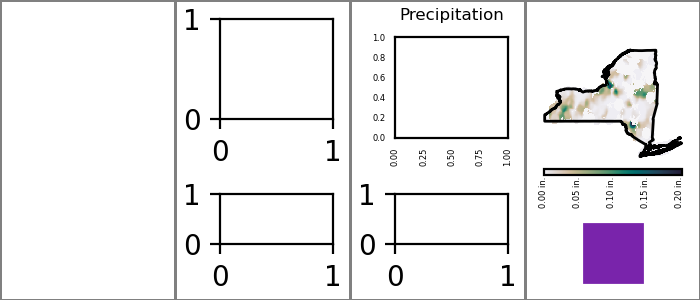
\includegraphics[width=1\columnwidth]{k_different_types.png}
  \caption{A topological representation of the data (in purple) is a simplified representation of how the records in a dataset are connected. Discrete rows of a table are discrete points, a 1D continuous function is evaluated on a 1D continuous interval, and a map is 2D continuous surface. }
\end{figure}
The topological properties of a dataset are the ways in which elements are organized, as described by Wilkenson\cite{wilkinsonGrammarGraphics2005}. Some examples, as shown in \autoref{fig:related-work:continuity:ktypes} are discrete rows of a table, a continuous 1D line, or a surface. The topological space (in purple) and the data form a key-value pair, as described by Munzner \cite{munznerVisualizationAnalysisDesign2014}. She imbues semantic meaning to the topology, wherein the key is an independent attribute used as a look up key to retrieve the value in the dataset. She defines the value as a dependent attribute. In this work we use a more general notion of the topological space as an indexing space for the data records. For example the data record in the yellow row in \autoref{fig:related-work:continuity:ktypes} can be expressed as a constant function of the yellow dot; A point on the green line is mapped to by evaluating the gaussian on a point on the interval; and each pixel in the map can be found via a lookup on the 2D surface. This general formulation of topology gives us a language for expressing the continuity of a dataset. 

\begin{figure}[h!]
  \label{fig:related-work:continuity:borked}
  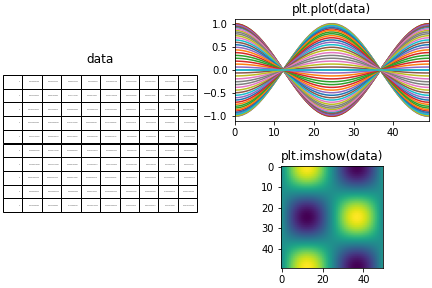
\includegraphics[width=1\columnwidth]{continuity.png}
\end{figure}
The continuity matters to visualization libraries because visual algorithms, such as a the line plot and image plot in \autoref{fig:related-work:continuity:borked}, assume that the continuity of their data, as described in taxonomies of visualization algorithms by Troy, M\"{o}ller, and Chi \cite{toryRethinkingVisualizationHighlevel2004,chiTaxonomyVisualizationTechniques2000}. In \autoref{fig:related-work:continuity:borked}, both algorithms are fed the same input matrix. The line plot assumes this matrix is a list of lines and plots it as such. The image map assumes that the data is an image and plots it as such. Neither function has a way of asking the matrix what it is, nor does the matrix encode information about the continuity of the data it contains. While this work is not about choosing the right visualization type for the given continuity, the ability to encode the continuity expectations in the visual algorithm and the data container would provide a way of ensuring that the assumptions match. 

Current visualization libraries handle continuity in two main ways. Libraries that provide "building block" \cite{wongsuphasawatNavigatingWideWorld2021} components for building new visual algorithms embed their assumptions in their algorithms. This flexibility allows libraries such as matplotlib\cite{hunterMatplotlib2DGraphics2007}, VTK\cite{hanwellVisualizationToolkitVTK2015,geveciVTK2012}, and D3\cite{bostockDataDrivenDocuments2011} to support a wide variety of data types, but at the cost of the ambiguity of \autoref{fig:related-work:continuity:borked}. These libraries can also have visual algorithms with  parameters that are tuned to the expected data in a way that leaves the over all library feeling uncohesive. On the other hand, domain specific libraries are designed with the assumption of continuities that are common in the domain \cite{HeerSoftware2006}. Tabular data is a very common data topology and is assumed by 
A Presentation Tool\cite{mackinlayAutomatingDesignGraphical1986, mackinlayAutomatingDesignGraphical1986} and grammar of graphics\cite{wilkinsonGrammarGraphics2005} and the ggplot\cite{wickhamGgplot2ElegantGraphics2016a}, vega\cite{satyanarayanDeclarativeInteractionDesign2014}, and altair\cite{vanderplasAltairInteractiveStatistical2018} libraries built on these frameworks. Image libraries such as Napari\cite{nicholas_sofroniew_2021_4533308} and ImageJ\cite{schneiderNIHImageImageJ2012} and its humanaties data ImagePlot\cite{studiesCulturevisImageplot2021} plugin assumed that the input is 2D continuous. Networking libraries such as gephi\cite{bastianGephiOpenSource2009} and networkx\cite{HagbergExploringNetwork2008} assume a graph like structure. These libraries tend to benefit from more cohesive apis, but at the cost of a much more limited set of visualization algorithms than the building block libraries. 

\note{maybe move the following to \autoref{sec:atct:io} and consolidate?}
To bridge the need for flexibility and cohesiveness, we build on the proposal of fiber bundles as a general abstraction model for visualization data, as proposed by Butler\cite{butlerVectorBundleClassesForm1992,butlerVisualizationModelBased1989}. Fiber bundles are a mathematical structure that can be used to encode the topological properties of visualization data. There is also a methodology for encoding field types in fiber bundles, as described in Spivak's description of tables as fiber bundles\cite{spivakSIMPLICIALDATABASES}. Fiber bundles are discussed in more detail in \autoref{sec:atct:fiber-bundles}, but broadly they provide a mathematical representation of data that can encode topological properties, field types, and data values in a way that is both uniform and continuity and dimension independent way. 

\subsection{Equivariance}
Equivariant maps are functions where variations in the input match variations in the output. The expectation that visualizations are equivariant maps from data to visual representation was first formalized by Bertin \cite{bertinSemiologyGraphicsDiagrams2011a}. He classified datasets into point, line, and surface topologies and proposed that these datasets should be represented by visual elements with the same sort of topology - points should be represented by discrete entities, lines by lines, and surfaces through area marks. Bertin also codified the idea that visual encoding of a data field should match the structure of the field; for example ordered data should be encoded as an ordered visual element or quantitative data as a quantitative visual element. This structure mapping is necessary to ensure that the visual representations in graphs are not distorting the data\cite{tufteVisualDisplayQuantitative2001} and graphs are easier to understand when properties match \cite{norman_things_smart}.

The expectation of matching structure is generalized as a mapping of a binary operator that acts on the data domain to a binary operator that acts on the graphic domain by Mackinlay\cite{mackinlayAutomaticDesignGraphical1987} An invertible binary operator is the basis of Kindlemannn and Scheideggers's algebraic model of visualization\cite{kindlmannAlgebraicProcessVisualization2014}. They propose three specific types of equivariance: that the visualization should not change if the data representation (i.e. the data container) changes, that changing the data should change the visualization in the same way in a perceptually significant manner. While the data representation introduced in \autoref{sec:atct:io} dispenses with a distinction between containers and the data, the definition of equivariance introduced in  \autoref{sec:artist:equivariance} includes invariant transformations and visually measurable transformations. 

Visualization libraries are in part measured by how expressive the components of the library are; expressiveness is a measure of which structure preserving mappings a tool can implement \cite{mackinlayAutomaticDesignGraphical1987}. While some visualization tools aim to automate the pairing of data with structure preserving automated tool, such as Tableau\cite{StoltePolaris2002,hanrahanVizQL2006,MackinlayShowme2007}, many visualization libraries leave that choice to the user. Some libraries, such as Matplotlib, set default encoders for their visual algorithms and allow the user to change the default. In this work, we propose guidelines for building expressive structure informed data to visual transformers. As with visual algorithms, we aim to provide a way to check that the structure of the data matches the structure expected by the component. Doing so allows users to more easily develop equivariant visual algorithms.

\section{Bundles and Sheaves}
\label{sec:atct}
A goal of this work is to develop guidelines for building composable structure preserving functions for translating data into visual representations. Concepts in algebraic topology and category theory provide a language for formally expressing the structure that these visualizations are expected to preserve. Fiber bundles and sheaves, which come from algebraic topolology, provide a uniform generalizable way to describe data and visualization. Category theory is a method to describe how objects are specified, constrained, and composed \cite{wielsManagementEvolvingSpecifications1998}\; therefore in this work we propose categorical constructions of visualization components as specifications for implementable components. A brief introduction to category theory for visualization practitioners is in Vickers et al \cite{vickersUnderstandingVisualizationFormal2013}, but they are applying category theory to semantic concerns about visualization design rather than library architecture.

\subsection{Fiber Bundles}
\label{sec:atct:fiber-bundles}
Fiber bundles, are a "unified, dimension-independent framework", as described by Butler\cite{butlerVectorBundleClassesForm1992,butlerVisualizationModelBased1989}, that allow us to seperatly describe the topological properties and fields of a data source and also the mapping between topolology and data values. A fiber bundle $(\dtotalc, \dbasec, \pi, \dfiberc)$ is a structure with topological spaces $\dtotalc, \dfiberc, \dbasec$ and continuous surjective map $\pi: \dtotalc \rightarrow \dbasec$\cite{FiberBundle2020}. 

\begin{equation}
  \label{eq:atct:fb:intro}
  \begin{tikzcd}[ampersand replacement=\&, row sep=huge]
   \dfiberc
    \arrow[r, hook, color=total] \& 
    \dtotalc
    \arrow[d, "\pi"',color=total] \\
     \& 
  \dbasec
     \arrow[u, "\dsectionc"', bend right, pos=.5, color=section]
  \end{tikzcd}
\end{equation} 

The \textcolor{base}{base space} is a topological space \dbasec\ with points $\dbasepointc \in \dbasec$ and topology $\mathcal{T}_{\dbasec}$; $\mathcal{T}_k$ is a set of opensets $ \dbasepointc \in \opensetc \subseteqq \dbasec$ \cite{munkresElementsAlgebraicTopology1984} that cover the base space \dbasec.  The \textcolor{fiber}{fiber space} is a topological space \dfiberc\ that is the preimage of the projection function $\pi$ at a point in the base space $\dfiber_{\dbasepointc} = \pi^{-1}(\dbasepointc)$ and fibers of a bundle are isomorphic $\dfiberc \simeq \dfiberc_{\dbasepointc}\;\forall \dbasepointc \in \dbase$. The \textcolor{section}{sections} of a bundle $\dsection$ are maps from the base space to points in the bundles over that base space $\textcolor{set}{\Gamma}$ denotes the set of all sections in a bundle over an openset. 
\begin{equation}
  \label{eq:atct:fb:sections}
  \cgamma{\opensetc}{\dtotalc\restriction_{\opensetc}} \coloneqq \big\{\dsectionc: \opensetc\rightarrow \dtotalc\restriction_{\opensetc} \; \bigm{\vert} \pi(\dsectionc(\dbasepointc)) = \dbasepointc\;for\, all\; \dbasepointc \in \opensetc \big\} 
\end{equation}
 
A fiber bundle is locally trivial, which means that for every point \dbasepointc\ there exists an open neighborhood $\dbasepointc \in \opensetc \subseteq \dbasec$ such that there is a homeomorphism $\pi^{-1}(\opensetc)\xrightarrow{\equivc} \opensetc \times \dfiberc$. A bundle may be globally trivial, meaning that $\dtotalc = \dbasec \times \dfiberc$, and generally can be thought of as a twisted product of total and base spaces \cite{munkresElementsAlgebraicTopology1984}. Throughout this work we will assume that fiber bundles are trivial because that allows us to model the section functions as from $\texttt{base} \rightarrow \texttt{fiber}$ since the fiber is the same at all points in the base space. 

Fiber bundles can be used to model data for visualization, as proposed by Butler\cite{butlerVectorBundleClassesForm1992, butlerVisualizationModelBased1989}. We describe the topological properties of the data \cite{wilkinsonGrammarGraphics2005} as the base space \dbasec. The topological properties, as described by Wilkenson, are how the data is organized - for example \dbase\ could be discrete points, a line, a 2D surface, a 3D volume, or a graph. The names and data types of the data fields can be expressed as the fiber space \dfiberc, as described by Spivak \cite{spivakDatabasesAreCategories2010,spivakSIMPLICIALDATABASES}. Extending Spivak's fiber bundle description of a table, we define the values returned by a section as named and typed records of the dataset. 

\begin{figure}[h!]
  \label{fig:atct:fb}
  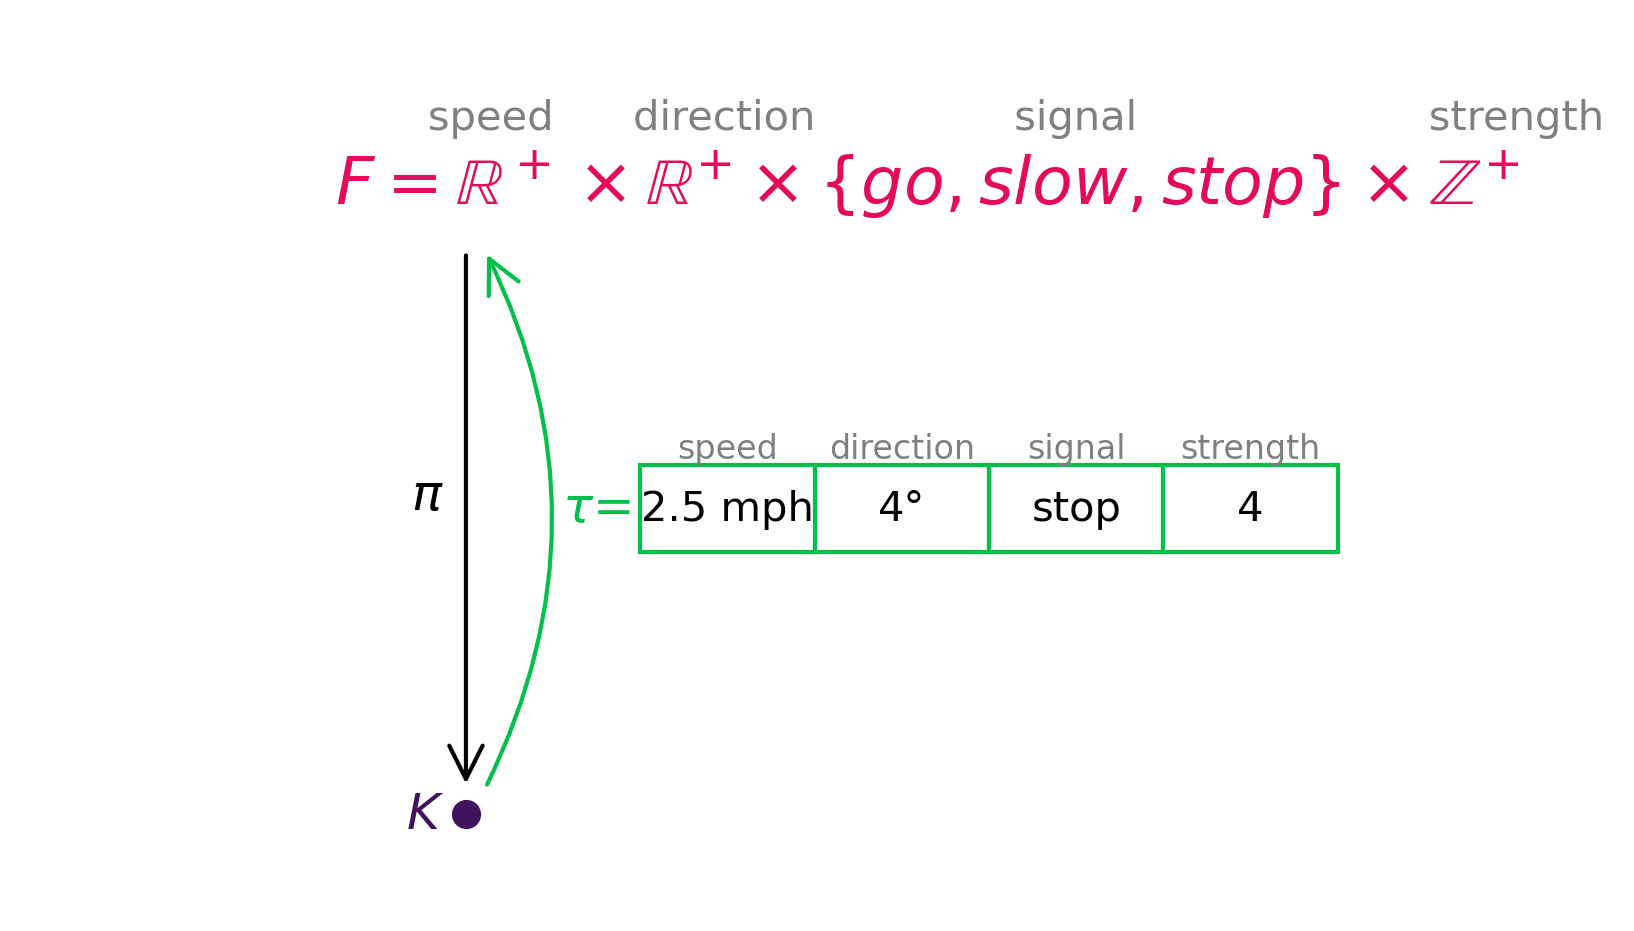
\includegraphics[width=\columnwidth]{fb_tau.png}
  \caption{This trivial dataset consists of a single point $\dbasec$ and the fields \texttt{speed, direction, signal, and strength}. Each of these fields has an associated datatype, which is the set of possible valid values for that field. The fiber space is the cartesian product of these sets $\dfiberc$. Each section $\dsectionc$ function returns a single record in the fiber, here the data record outlined in green.  
  \note{maybe change to temperature}}
\end{figure} 
A fiber bundle is a mathematical structure for encoding continuity, type, and datasets with that continuity and type. In \autoref{fig:atct:fb}, the continuity is a discrete point \dbase. The fiber space that encodes the types is the cartesian product of the field types, and the section returns a single record with values of each field type. While this is a very trivial example, a fiber bundle base space can have almost any topology. The fiber space also does not really have restrictions on which types it can encode or the structure of those types - for example, \texttt{speed} and \texttt{direction} are separate fibers in \autoref{fig:atct:fb} but can be combined into a single two dimensional fiber $\dfiber_{speed, direction} = {\mathbb{R}^{+}}^{s}$ The generality in base space and fiber space makes fiber bundles a unified dimension and type independent data abstraction that can encode most of the common visualization data set structures, such as continuous functions, tables, data cubes, images and networks. 

We also use fiber bundles to represent the output of a visualization algorithm, which we term the graphic but generalizes to output on any display space, such as a screen or 3D print. 
\begin{equation}
  \label{eq:atct:fb:graphic}
  \gfiberc \hookrightarrow \gtotalc \xrightarrow{\pi} \gbasec
\end{equation}
The base space \gbasec\ is a parameterization of the display area, for example the inked bounding box in cairo \cite{CairographicsOrg}. The fiber space \gfiberc\ is an abstraction of the renderer fields, for example $\{x,\,y,\,r,\,g,\,b,\,a\}$. The sections of the graphic 
\begin{equation}
  \label{eq:atct:fb_graphic_section}
  \cgamma{\opensetgc}{\gtotalc\restriction_{\opensetgc}} \coloneqq \big\{\gsectionc: \opensetgc\rightarrow \gtotalc\restriction_{\opensetgc} \; \bigm{\vert} \pi(\gsectionc(\gbasepointc)) = \gbasepointc\;for\, all\; \gbasepointc \in \opensetgc \big\}
\end{equation}
are functions that generate different graphics, for example markers for a scatter plot, bars for a bar chart, cells of a heatmap, or pixels of an image.


\begin{figure}[h!]
  \label{fig:atct:fb:graphic}
  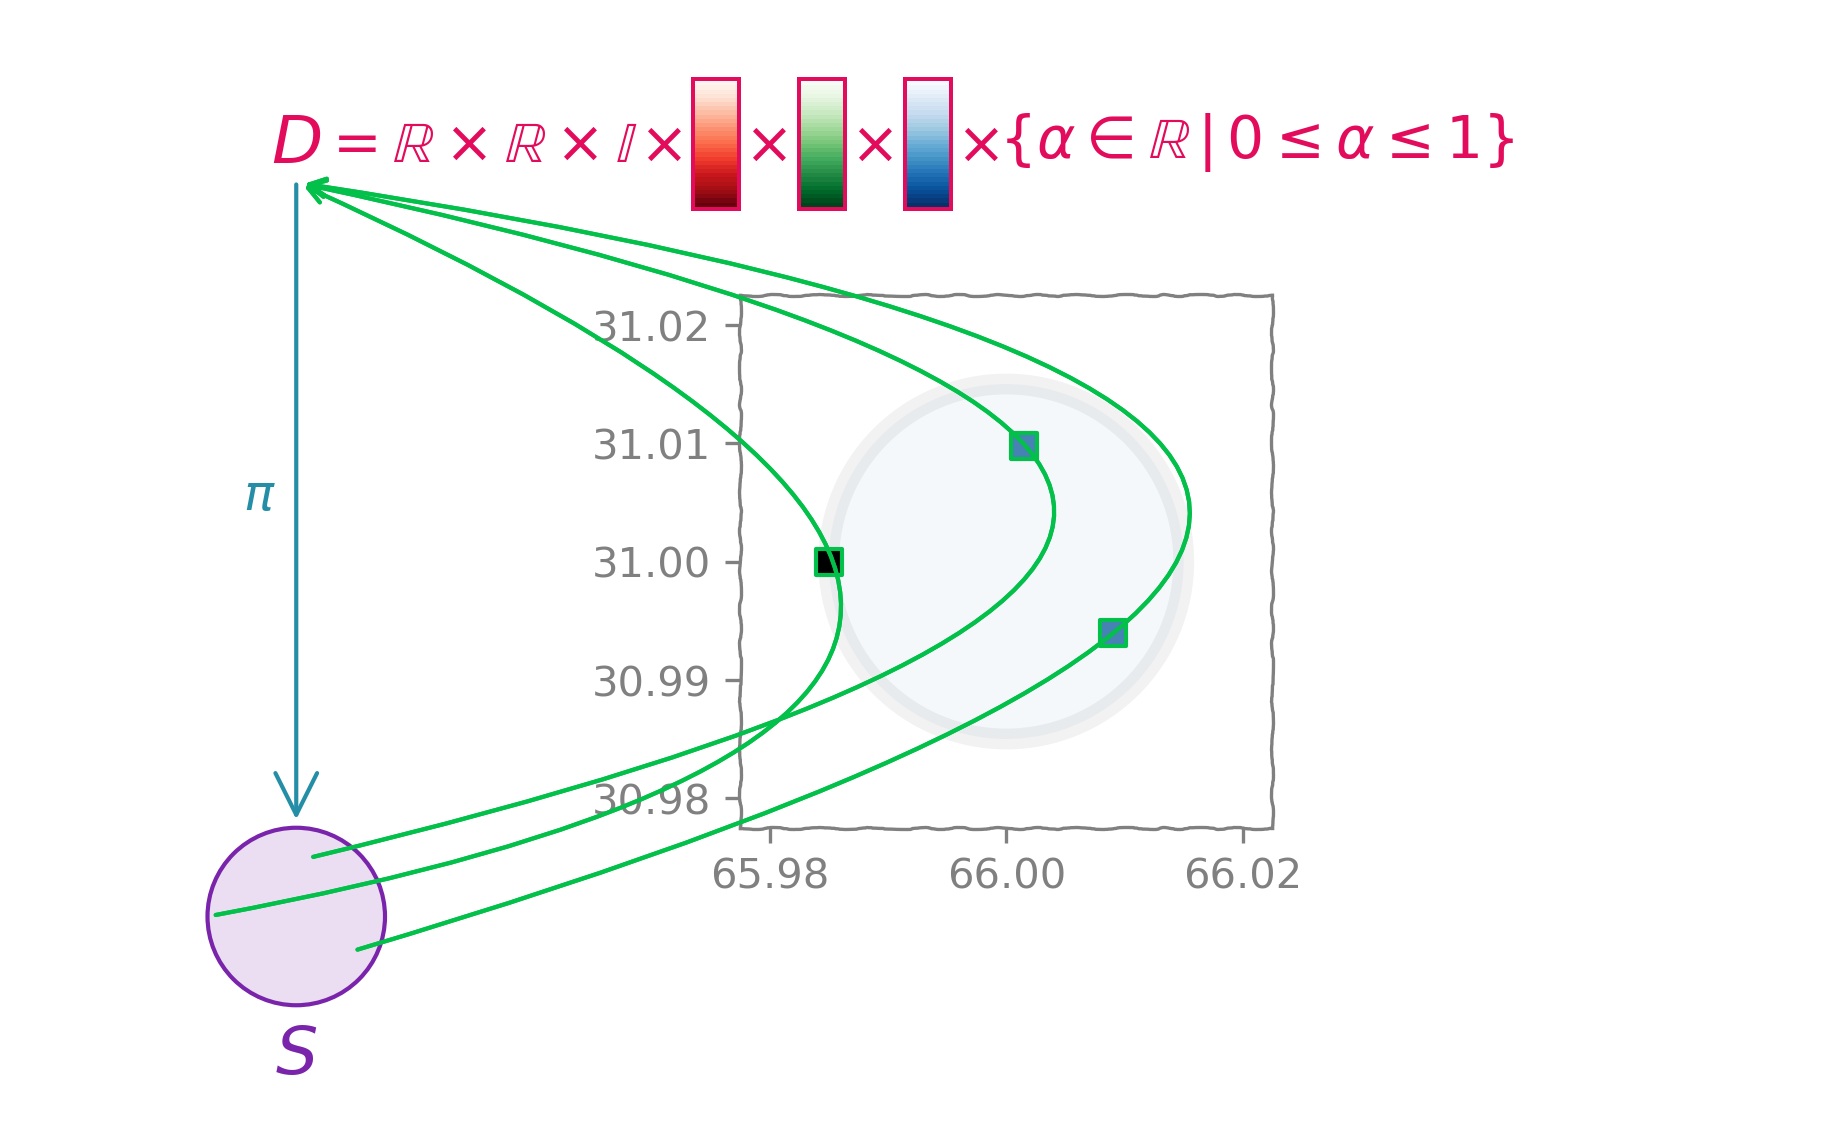
\includegraphics[width=1\columnwidth]{fb_rho.png}
  \caption{A bundle representation of a section that generates a scatter marker on a 2D screen. The fiber space encodes the potential color and position of each pixel in a prerender space. The marker is a 2d graphic; therefore the base space that parameterizes the graphic area \dbasec\ is a 2d disc. This section \gsection\ describes how to build a square red marker; a section evaluated on a single point $\gbasepoint \in \gbase$ is an infinitesimally small piece of the square, here illustrated as the small piece of the square outlined in green.}
\end{figure}

In \autoref{fig:atct:fb:graphic}, the section function $\gsection$ encodes the drawing of a red square marker. The renderer subsamples the position fibers  \textit{x} and \textit{y} of the graphic fiber space \gfiber. The preimage of the section at these coordinates returns a set of coordinates \({\gsection^{-1}_{x,y}} = \{\gbasepoint | \gsection(\gbasepoint)\restriction_{x,y} = \(x,y\)\}\) at the points \(\gbasepoint \in \gbase\) in the graphic base topological space. The section is then evaluated at these points \(\gsection\restriction_{\gsection^{-1}_{x,y}}\) to return a set of points in the fiber. One of these points, enlarged for visibility, is illustrated as the small square swatch inside the larger marker in \autoref{fig:atct:fb}. The renderer is handed some version of $\gsection$ to produce the final graphic. 

\subsection{Input and Output Types}
\label{sec:atct:io}
As described in \autoref{sec:atct:fiber-bundles}, we model data as a map from base space to fiber space.To encapsulate the structure carried in these maps, and provide a way to define these maps in reusable and composable manner, we define categories of base and fiber spaces. 

\begin{definition}
  \label{sec:atct:io:base}
  The base space category $\mathcal{\opensetc}$ has open set objects $\opensetc$ and inclusion morphisms $\iota: \opensetc_1 \rightarrow \opensetc_2$ such that $\opensetc_1 \subseteq \opensetc_2$. 
\end{definition}

By definition, each object in a category has an identity morphism and morphisms are associative and commutative \cite{barrCategoryTheoryComputing}. 

\begin{definition}
  \label{def:atct:io:fiber}
  The fiber category $\mathcal{\dfiberc}$ is a monoidal category, meaning the category has a single object $\dfiberc$ of an arbitrary type. The morphisms on the fiber object are $\dfunctc \in Hom(\dfiberc, \dfiberc)$. 
\end{definition}

The fiber category is equipped with a bifunctor $\otimes: \mathcal{\dfiber} \times \mathcal{\dfiber} \rightarrow \mathcal{\dfiber}$. The bifunctor provides a method for combining fibers, thereby allowing for fields that contain multityped values. For example, RGB color can either be represented as three fiber fields $\dfiber_{red}, \dfiber_{green}, \dfiber_{blue}$ or a composite fiber field $\dfiber_{red} \otimes \dfiber_{green} \otimes \dfiber_{blue} = \dfiber_{RGB}$.

\subsection{Sheaves}
\label{sec:atct:sheaves}
Sheaves on bundles are an "algebraic data structure", as described by Ghrist \cite{ghristElementaryAppliedTopology2014}, for expressing the bookkeeping involved in keeping track of sections of data over opensets. Sheaves are a way of expressing that subsets, distributed data, and streaming data are local sections that can be glued together. Formally, pre-sheaves are functors, meaning they are functions from objects of one category to objects of another category \cite{WhatFunctorDefinitions}. Here the sheaf 
\begin{equation}
  \label{eq:atct:sheaf:functor}
  \sheafc_{\dbasec, \dtotalc}: \opensetc \rightarrow \cgamma{\opensetc}{\dtotalc\restriction_{\opensetc}}
\end{equation}
denotes a sheaf from opensets on the base space $\dbase$ to sets of sections on the bundle $\dtotal$. As a contravariant functor it preserves morphism s

\begin{equation}
  \label{eq:atct:presheaf}
  \begin{tikzcd}
    \cgamma{\opensetc_1}{\dtotalc\restriction_{\opensetc_1}}  &  & \cgamma{\opensetc_2}{\dtotalc\restriction_{\opensetc_2}} 
    \arrow[ll, "\iota^*"', maps to, color=set] \\
    & & \\
    \opensetc_1 
    \arrow[rr, "\iota", maps to, color=base] 
    \arrow[uu, "{\sheafc_{\dbasec, \dtotalc}}", maps to, color=sheaf] &  & \opensetc_2 
    \arrow[uu, "{\sheafc_{\dbasec, \dtotalc}}"', maps to, color=sheaf]              
    \end{tikzcd}
\end{equation}

which associates a set of sections $\cgamma{\openset}{\dtotal\restriction_{\openset}}$ with an openset \openset. The sets of sections are objects of the category \setc\ and the morphisms of the category are restrictions\footnote{restriction functions } $\iota^*$. The sheaf over a an open set $\openset$ surrounding a point $\dbasepoint$ is called a stalk\cite{StalkSheaf2019}
\begin{equation}
  \label{eq:atct:sheaf:stalk}
    \sheaf_{\dbase, \dtotalc}\restriction_{\dbasepoint}\coloneqq \lim\limits_{\openset\ni \dbasepoint} \Gamma(\openset, \dtotal\restriction_{\openset}) 
\end{equation}
where the fiber is contained inside the stalk  $\dfiber_{\dbasepoint} \subset  \sheaf_{\dbase, \dtotal}\restriction_{\dbasepoint}$. The germ is the section evaluated at a point in the stalk  $\dsection(\dbasepoint) \in \sheaf_{\dbase, \dtotal}\restriction_{\dbasepoint}$ and is the data. \note{I never use stalk and germ terminology at any point in this paper}
 
A sheaf is a presheaf that satisfies the locality and gluing axioms \cite{bakerMathsSheaf}. 
\begin{definition}
\label{def:atct:sheaf:locality}
The locality axiom is that given a union of opensets $\mathscr{\opensetc} = \bigcup\limits_{i\in I} \opensetc_i$ and $\dsectionc^{a}, \dsectionc^{b} \in \sheafc(\mathscr{\opensetc})$,  if $\dsectionc^{a}\restriction_{\opensetc_i} = \dsectionc^{b}\restriction_{\opensetc_i}$ for each $\opensetc_i \in \opensetc$ then $\dsectionc^{a} = \dsectionc^{b}$
\end{definition}
This means that two sections in a sheaf are equal when they evaluate to the same values over all open sets in a collection. 
\begin{definition}
\label{def:atct:sheaf:gluing}
The gluing axiom is that given $\dsectionc^{i} \in \sheafc(\opensetc_i)$ such that ${\dsectionc^{i}}\restriction_{\opensetc_i\cap \opensetc_j} = {\dsectionc^{j}}\restriction_{\opensetc_i \cap \opensetc_j}$ for $\opensetc_i, \opensetc_j \in \mathscr{\opensetc}$, there exists $\dsectionc \in \sheafc(\mathscr{\opensetc})$ such that $\dsectionc\restriction_{\opensetc_i} = {\dsectionc^{i}}$. 
\end{definition}
This means we can construct a section $\dsection$ on the collection of open sets that is the union of sections defined on specific open sets. This expresses an equivalency between a concatenated representation of data and the distributed representation of the same data. In this model, we represent data and graphics as a sheaf; doing so allows us to express that data sources are expected to implement the bookkeeping that a sheaf requires, meaning inclusions, restrictions, locality, and gluing must be preserved. 

\subsubsection{Structure}
\label{sec:atct:sheaves:measurments}
We define structure on data as the allowable \textcolor{action}{transformations on the bundle}, which we formalize as actions $\dfuncc$ on sections of that sheaf. Our construction of $\dfunc$ is a generalization of the classification of measurement scales by their mathematical structure \cite{stevensTheoryScalesMeasurement1946,leaFormalizationMeasurementScale, thomasMathematizationNotMeasurement2014}, which often serves as the basis of the equivariance described in \autoref{sec:related-work:equivariance}.

We separate data transformations into two types, transformations on the base space $(\dfunchc, \dfuncpullc)$ and transformations on the fiber space $\dfunctc$. 
\begin{equation}
  \label{eq:atct:sheaves:monoid_morphism}
  \begin{tikzcd}
    \cgamma{\opensetc}{\dtotalc\restriction_{\opensetc}} 
    \arrow[rr, "\dfuncpullc", color=action, maps to] &  & 
    \cgamma{\opensetc^{\prime}}{\dfuncpullc\dtotalc\restriction_{\opensetc^{\prime}}} & 
    \cgamma{\opensetc^{\prime}}{\dfuncpullc\dtotalc\restriction_{\opensetc^{\prime}}} 
    \arrow[dd, "\dfunctc", color=action] \\
     &  & &       \\
    \opensetc 
    \arrow[uu, maps to,color=sheaf]  &  & \opensetc^{\prime} 
    \arrow[ll, "\dfunchc"', color=action, maps to] 
    \arrow[uu, maps to, color=sheaf] & \cgamma{\opensetc^{\prime}}{\dfuncpullc\dtotalc\restriction_{\opensetc^{\prime}}}                       
    \end{tikzcd}
\end{equation}
As shown in \autoref{eq:atct:sheaves:monoid_morphism}, the base space transform 
\begin{equation}
 \label{eq:atct:morphism:base}
\dfunch: \openset^{\prime}\rightarrow \openset
\end{equation}
is from one open set to another open set in the same base space $\openset, \openset^{\prime} \subseteq \dbase$. For example a remapping of an underlying indexing, such as a sorting of primary keys for a database of discrete values. This base space transformation induces a pullback section 
\begin{equation}
  \label{eq:atct:morphism:basepull}
  \dfuncpull \dsection \restriction_{\openset^{\prime}}: \dsection\restriction_{\openset^{\prime}} \mapsto \dsection \restriction_{\openset^{\prime} \circ \dfunch} 
\end{equation}
such that $\dsection|_{\openset} = \dfuncpull\dsection|_{\opensetc^{\prime}}$ because $\dsection|_{\openset} = \dsection|_{\dfunch(\opensetc^{\prime})}$. This means that the base space transformation \dfunch\ does not change the data values at a given point
\begin{equation}
  \label{eq:atct:morphism:verify_base}
  \dsection(\dbase) = \dfuncpull\dsectionc(\dbasepoint^{\prime}) = \dsection(\dfunch(\dbase^{prime}))
\end{equation} 
where $\dfunch(\dbasepoint^{\prime}) = \dfunch(\dbasepoint)$. As introduced in \autoref{def:atct:io:fiber}, the fiber transformation $\dfunct: \dfuncpull \dtotal_{\dbasepoint^{\prime}} \rightarrow \dfuncpull \dtotal_{\dbasepoint^{\prime}}$ is a morphism on the fiber $\dfunct \in Hom(\dfuncpull\dfiber\restriction_{\dbasepoint^{\prime}},\dfuncpull\dfiber\restriction_{\dbasepoint^{\prime}})$ restricted to a point $\dbasepoint^{\prime} \in \openset^{\prime}$. The fiber transformation is a change in section 
\begin{equation}
  \label{eq:atct:morphism:fiber}
  \dfunct: \dfuncpull \dsection \restriction_{\openset^{\prime}} \mapsto \dfuncpull \dsection^{\prime} \restriction_{\openset}
\end{equation}
where $\dsection, \dsection^{\prime} \in \Gamma(\openset^{\prime}, \dfuncpull\dtotal\restriction_{\openset^{\prime}})$. Examples of a fiber transformation are actions such as partial ordering for ranking purpose \cite{bruggemannRankingPrioritizationMultiindicator2011} and the permutation, ordering, translation, and scaling codified as Steven's measurement scales \cite{stevensTheoryScalesMeasurement1946}. 

We define a full data transformation as one that induces both a remapping of the index space and a change in the data values
\begin{equation}
  \label{eq:atct:morphism:all}
  \dfuncc: \dsectionc\restriction_{\opensetc} \mapsto \dsectionc^{\prime}\restriction_{\opensetc} \circ \dfunchc
\end{equation}
which gives us an equation that can express complex transformations. For example, wind vectors on a sphere are a non-trivial bundle, meaning their fibers aren't identical at every point in the base space; therefore a rotation (change of base space) of the sphere must include an adjustment to the values that have moved closer to the pole (a change in fiber).  
The data transform \dfunc\ is composable 
\begin{equation}
  \dfuncc = (\dfunchc, \prod\limits_{i=0}^{n}\dfunctc_i)
\end{equation}
if each (identical) component base space is transformed in the same way $\dfunch$ and there exists functions $\dfunc_{a,b}: \dtotal_a \times \dtotal_b \rightarrow \dtotal_a \times \dtotal_b$, $\dfunc_{a}: \dtotal_a \rightarrow \dtotal_a$ and $\dfunc_{b}: \dtotal_b \rightarrow \dtotal_b$ such that $\pi_a \circ \dfunc_a = \dfunc_{a,b} \circ \pi_a$ and $\pi_b \circ \dfunc_b = \dfunc_{a,b} \circ \pi_b$ then $\dfunc_{a,b} = (\dfunc_a, \dfunc_b)$. This allows us to define a data transform where each fiber transform $\dfunct_{i}$ can be applied to a different fiber field $\dfiber_i$. 

\begin{figure}[h!]
  \label{fig:atct:phi}
  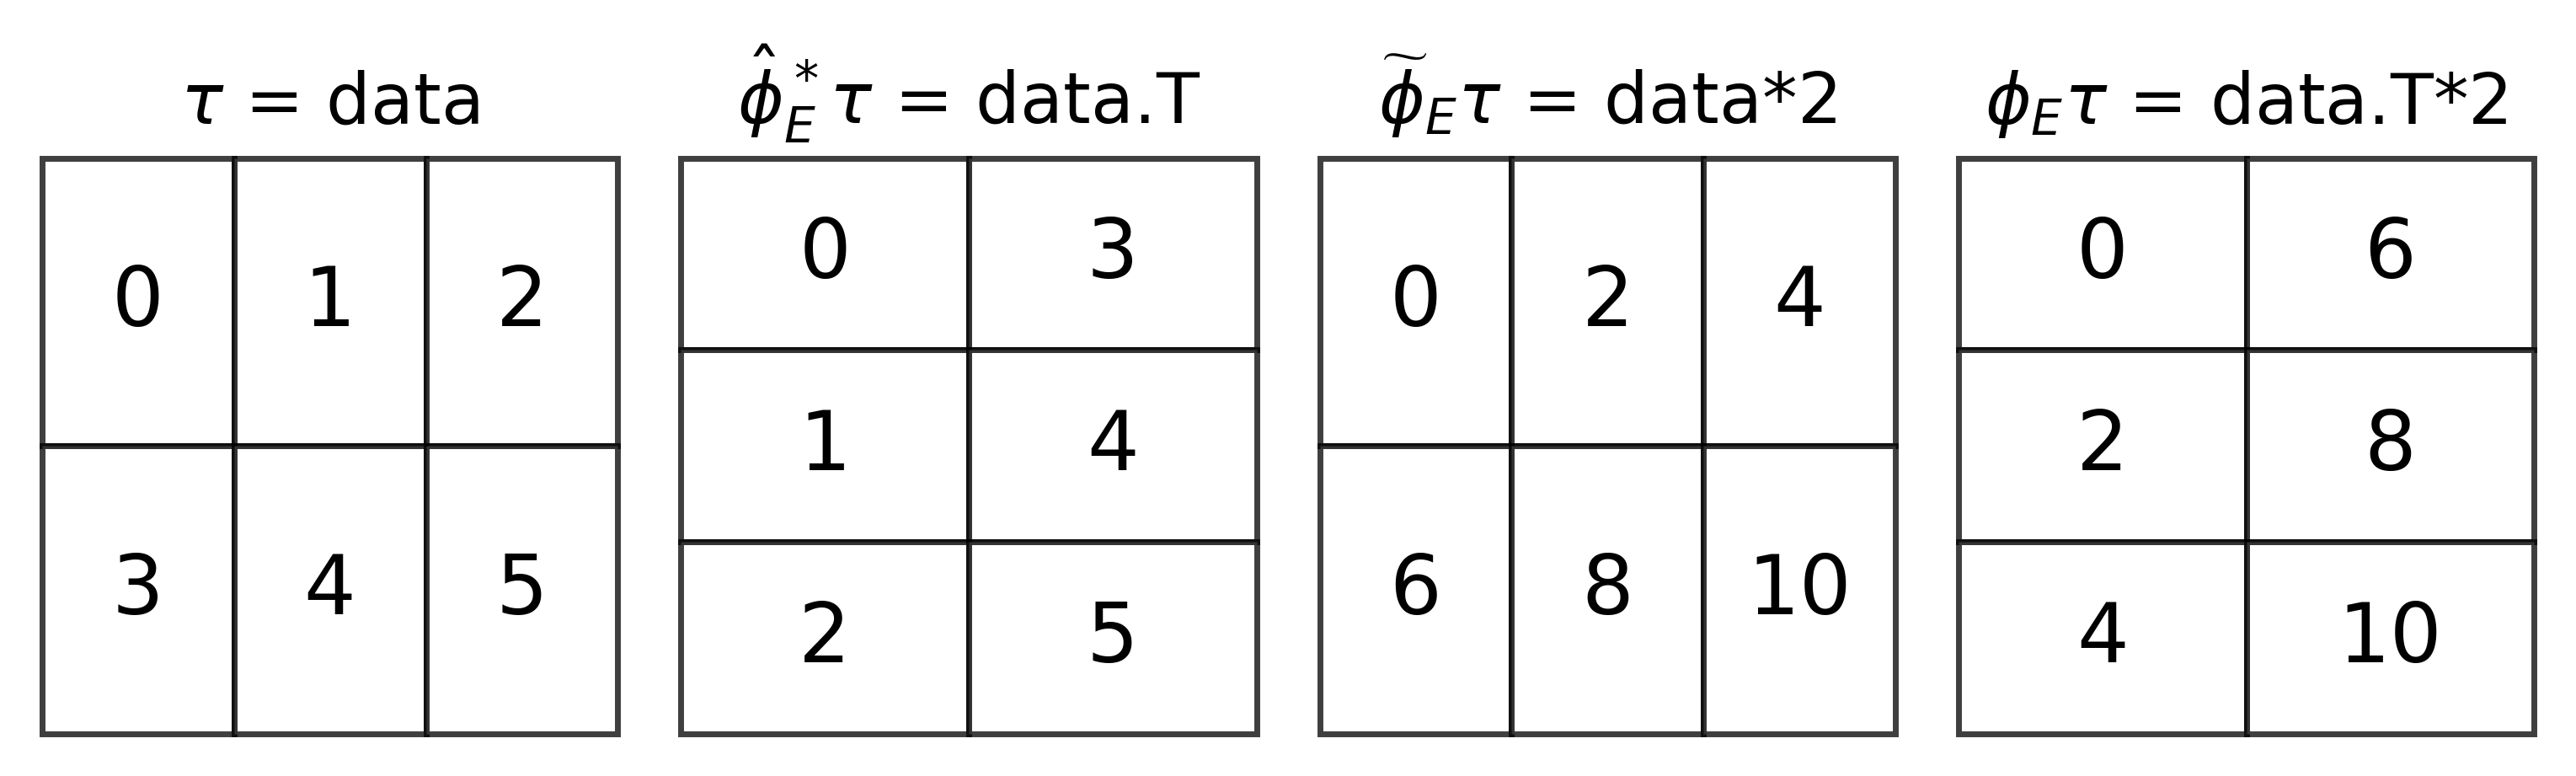
\includegraphics[width=\columnwidth]{phi.png}
  \caption{Values in a data set can be transformed in three ways: $\dfunch$-values can change position, .e.g transposed;  $\dfunct$-values can change, e.g. doubled; $\dfunc$ - values can change position and value}
\end{figure}
\autoref{fig:atct:phi} provides an example of a base space change \dfunch, a fiber space change \dfunct, and a composition of the two \dfunc\ applied to each data point $x_{\dbasepoint} \in \texttt{data}$. As defined in \autoref{eq:atct:morphism:verify_base}, 
since transposition is a $(\dfunch, \dfuncpull)$, every data value $x_{\dbasepoint}$ must be equal to the value at the corresponding location in the transposed matrix $x_{\dbasepoint} = x_{\dbasepoint^{\prime}}, \dfunch(\dbasepoint^{\prime}) = \dbasepoint$ for all $x_{\dbasepoint^{\prime}} \in texttt{data.T}$ . In \autoref{fig:atct:phi}, this is demonstrated in the columns becoming rows such that there are no new values and each value retains the same neighboring values. As defined in \autoref{eq:atct:morphism:fiber} scaling is a transform $\dfunct$ that changes the value of each point but not its location. In \autoref{fig:atct:phi}, this means that $x_{\dbasepoint^{\prime}}= 2*x_{\dbasepoint}, \dbasepoint = \dbasepoint_{\prime}$ for all indices in \texttt{data}, \texttt{data.T}. As defined in \autoref{eq:atct:morphism:all} and illustrated in \autoref{fig:atct:phi}, these transformations can combine to yield a matrix that is both transposed and scaled such that $x_{\dbasepoint^{\prime}} = 2*x_{\dbasepoint}$ for all  
$\dfunch(\dbasepoint^{\prime}) = \dbasepoint$

\subsection{Image Functors}
\label{sec:atct:xi}
The data sections defined in \autoref{eq:atct:fb} are sections of sheaves, introduced in \autoref{sec:atct:sheaves}, over open sets $\openset \subseteq \dbase$ in a base space \dbase\ that encodes the topology of the data topology. The graphic sections, defined in \autoref{eq:atct:fb_graphic_section}, are sections of sheaves over open sets $\opensetg \subseteq \gbase$ in a base space \gbase\ that encodes the topology of the graphic. We propose that there exists a continuous \textcolor{functor}{map between topological spaces} \vindexc 
\begin{equation}
  \label{eq:atct:xi}
  \vindexc: \opensetgc \rightarrow \opensetc 
\end{equation}
such that every $\opensetg \subseteq \gbase$ must map to a corresponding set $\openset \subset \dbase$. 

Given the map between spaces \vindex\, a property of sheaves is that there exist image functors\cite{ImageFunctorsSheaves2021} functors \vindexpull\ and \vindexpush. The \textcolor{functor}{pullback functor} $\vindexpullc$ sends sheaves over $\dbase$ to $\gbase$ and the \textcolor{functor}{pushforward functor} $\vindexpushc$  sends sheaves over $\gbase$ to $\dbase$
\begin{equation}
  \label{eq:atct:morphisms:xi}
\begin{tikzcd}[row sep=huge]
  \cgamma{\opensetc}{\dtotalc\restriction_{\opensetc}} 
  \arrow[rr, "\vindexpullc", maps to, color=functor] &  & 
  \cgamma{\opensetgc}{\vindexpullc\dtotalc\restriction_{\opensetgc}}  \\
  \opensetc 
  \arrow[d, "{\vindexpushc\sheafc_{\gbasec,  \gtotalc}}", dashed, maps to, color=sheaf] 
  \arrow[u, "{\sheafc_{\dbasec, \dtotalc}}"', maps to, color=sheaf] &  & 
  \opensetgc 
  \arrow[d, "{\sheafc_{\gbasec, \gtotalc}}", maps to, color=sheaf] 
  \arrow[u, "{\vindexpullc\sheafc_{\dbasec, \dtotalc}}"', dashed, maps to, color=sheaf] 
  \arrow[ll, "\vindexc"', maps to, color=functor] \\
  \cgamma{\opensetc}{\vindexpushc\gtotalc\restriction_{\opensetc}} &  & 
  \cgamma{\opensetgc}{\gtotalc\restriction_{\opensetgc}} 
  \arrow[ll, "\vindexpushc"', maps to, color=functor]                                                         
  \end{tikzcd}
\end{equation}
such that there is an association between graphic sections \gsection\ that take as input \gbasepoint\ and data sections that take input \dbasepointc\ when $\vindex(\gbasepoint) = \dbasepoint$. 

The pull back $\vindexpullc$ transports sheaves of sections on $\openset \subseteq \dbase$ over $\opensetg \subseteq \gbase$
\begin{equation}
  \vindexpullc\dsectionc: \opensetgc \rightarrow \vindexpullc \dtotalc\restriction_{\opensetgc} \in \cgamma{\opensetgc}{\vindexpullc\dtotalc\restriction_{\opensetgc}} 
\end{equation}
such that there is a way to then look up what data values correspond with a graphic index
\begin{equation}
  \vindexpullc\dsectionc(\gbasepointc) = \dsectionc(\vindex(\gbasepointc)) = \dsectionc(\dbasepointc)
\end{equation}

 The pushforward $\vindexpushc$ transports sheaves of sections on $\opensetgc$ over $\openset$
 \begin{equation}  
  \vindexpushc\gsectionc: \opensetc \rightarrow \vindexpushc \gtotalc\restriction_{\opensetc} \in \cgamma{\opensetc}{\vindexpushc\gtotalc\restriction_{\opensetc}} 
\end{equation}
such that it provides a way to look up which graphic  corresponds with a data index
\begin{equation}
  \vindexpushc\gsectionc(\dbasepointc) = \gsectionc\restriction_{\vindexprec(\dbasepointc)} = \gsectionc(\gbasepointc)\;\forall \gbasepointc\in \vindexprec(\dbasepointc)
\end{equation}

Therefore, the continuous map $\vindex$ and transport functors $\vindexpull, \vindexpush$ allow us to express the correspondence between graphic section and data section. 

\begin{figure}[h!]
  \label{fig:atct:morphisms:sheaf}
  \includegraphics*[width=1\columnwidth]{xi_scatter.png}
  \caption{The base space functor $\vindexc$ is the mapping from each disc $\gbasec_i$ to it's corresponding point $\dbasepointc_i$. Over each point is a data record $\dsectionc$. The pullback function $\vindexpullc$ copies these records over $\gbase$ so that each piece of each marker knows the data associated with it. Each graphic disc has a corresponding graphic function $\gsectionc$. The pushforward function $\vindexpushc$ converts $\gsectionc$ into the visual parameters associated with each data point $\dbasepoint$.}
\end{figure}

Functors between sheaves are a way of expressing the bookkeeping involved in keeping track of which graphic section corresponds to which data section. This allows us to construct graphic specifications for each data index $\vindexpush\gsection$ and retrieve the data $\vindexpull\dsection$ for any graphic section generating any piece of a graphic. In \autoref{fig:atct:morphisms:sheaf}, the graphic specifications are the set of visual parameters associated with each point $\dbasepoint_i$. Each of these parameters describes the corresponding graphic $\gsectionc|_{\gbase_i}$ generated by evaluating the graphic section on the graphic base space associated with that data point $\vindexpre^{\dbasepoint_i} = \gbase_i$. The pullback functor $\vindexpull$ copies each data section at each point $\dsectionc(\dbasepointc_i)$ over the corresponding disk; in \autoref{fig:atct:morphisms:sheaf} this means that every pixel in a given marker, for example the yellow triangle, maps back into a single data record. Visualization specification languages such as vega \cite{heerDeclarative2010} and svg \cite{quintScalable2003} assume that there is a graphic  specification for every point. Interactive tooltips assume that there is a map between the graphics rendered on screen and the data such that a glyph maps back to a record. The functors $(\vindex, \vindexpush, \vindexpull)$ codify the expectation of these mappings between data and graphic space. 

We propose that visualization libraries implement morphisms from a data sheaf $\sheafc_{\dtotal, \dbase}$ to a graphic sheaf $\sheafc_{\gtotal, \gbase}$ 
\begin{equation}
  \label{eq:atct:sheaves:homset}
  \begin{tikzcd}
    \cgamma{\opensetc}{\dtotalc\restriction_{\opensetc}} 
    \arrow[dd, "\textcolor{set}{Hom}_{\sheafc_{\dbasec}}"', color=homset] 
    \arrow[rrdd, "\textcolor{set}{Hom}_{\sheafc_{\dbasec},\sheafc_{\gbasec}}", color=homset] 
    \arrow[rr, "\vindexpullc", color=functor] &  &
    \cgamma{\opensetgc}{\vindexpullc\dtotalc\restriction_{\opensetgc}} 
    \arrow[dd, "\textcolor{set}{Hom}_{\sheafc_{\gbasec}}", color=homset] \\
     & & \\
    \cgamma{\opensetc}{\vindexpushc\gtotalc\restriction_{\opensetc}} &  & 
    \cgamma{\opensetgc}{\gtotalc\restriction_{\opensetgc}} 
    \arrow[ll, "\vindexpushc"', color=functor]                  
    \end{tikzcd}
\end{equation}
and the hom set is the set of all morphisms from one sheaf to the other. The functors $\vindexpullc, \vindexpushc$ are adjoint, meaning that there is a functorial isomorphism \cite{harder2008lectures} such that 
\begin{equation}
  \label{eq:atct:sheaves:homset:functors}
\begin{split}
  & \textcolor{set}{Hom}_{\sheafc_{\gbasec}}(\vindexpullc\sheafc_{\dtotalc, \dbasec},\sheafc_{\gtotalc,\gbasec})\\
  \simeq & \textcolor{set}{Hom}_{\sheafc_{\dbasec}}(\sheafc_{\dtotalc, \dbasec},\vindexpushc\sheafc_{\gtotalc,\gbasec}) \\
  \simeq & \textcolor{set}{Hom}_{\sheafc_{\dbasec},\sheafc_{\gbasec}}(\sheafc_{\dtotalc, \dbasec},\sheafc_{\gtotalc,\gbasec}) \\
\end{split} 
\end{equation}
which means that the diagram of sheaf morphisms \autoref{eq:atct:sheaves:homset} is commutative; therefore the functors $\vindexpullc$ and $\vindexpushc$ can be used to adapt morphisms written over one space to another space. 
This provides us flexibility over which space to construct data to graphic transforms. For example, specifications such as svg\cite{quintScalable2003} and Vega\cite{satyanarayanDeclarativeInteractionDesign2014}, typically define their transformations in data space and return specifications for the render to evaluate. An artist may also want to specify the transformations in a proxy of graphic space, for example to generate on-demand dynamically resampled continuous lines.

\section{Artist: Data to Graphic}
\label{sec:artist}
In this work we propose that visualization libraries are implementing a subset of the functions in the hom sets in \autoref{eq:atct:sheaves:homset}. We call these subset of functions the artist:
\begin{align}
  \label{eq:artist:hom_transport}
  \vartistc:& \cgamma{\dbasec}{\dtotalc}\textcolor{artist}{\rightarrow} \cgamma{\gbasec}{\gtotalc} \in \textcolor{set}{Hom}_{\sheafc_{\dbase}, \sheafc_{\gbase}}\\
  \vartistc^{\dbasec}:&\cgamma{\dbasec}{\dtotalc}  \textcolor{artist}{\rightarrow} \cgamma{\dbase}{\vindexpushc\gtotalc} \in \textcolor{set}{Hom}{\sheafc_{\dbase}}\\
  \vartistc^{\gbasec}:& \cgamma{\gbasec}{\vindexpullc\dtotalc} \textcolor{artist}{\rightarrow} \cgamma{\gbasec}{\gtotalc} \in \textcolor{set}{Hom}_{\sheafc_{\gbase}}
\end{align}
 Because the artists can be constructed as morphisms of sheave over the same base spaces, as listed in \autoref{eq:atct:sheaves:homset:functors}, they are natural transformations
\begin{align}
  \label{eq:artist:natural_transform}
  \vartistc^{\dbasec}:& \sheafc_{\dbasec, \dtotalc} \textcolor{artist}{\Rightarrow} \vindexpushc \sheafc_{\gbasec, \gtotalc}\\
  \vartistc^{\gbasec}:&\vindexpullc\sheafc_{\dbasec, \dtotalc} \textcolor{artist}{\Rightarrow}\sheafc_{\gbasec, \gtotalc}
\end{align}
which means that they are maps of functors that take the same input object and return objects in the same category\cite{milewskiCategoryTheoryProgrammers}. As illustrated in \autoref{eq:atct:sheaves:homset}, the sheaf functors
\begin{equation}
  \label{eq:artist:sheaf:base}
    \begin{tikzcd}
      \cgamma{\dbasec}{\dtotalc} &  & \dbasec \arrow[ll, "{\sheafc_{\dbasec, \dtotalc}}"', maps to, color=sheaf] \arrow[rr, "{\vindexpushc\sheafc_{\gbasec, \gtotalc}}", maps to, color=sheaf] &  & \cgamma{\dbase}{\vindexpushc\gtotalc} 
      \end{tikzcd}
\end{equation}
take as input the same object \opensetc\ and return sets of data and graphic sections that are objects in \setb. As a map between these sheaf functors, the artist has to preserve the $\iota, \iota^*$ morphisms of the presheaf functor, described in \autoref{eq:atct:presheaf}, such that the following diagram commutes

\begin{equation}
  \label{eq:artist:natural_transform:inclusions}
  \begin{tikzcd}
    \dbasec_1 & \cgamma{\dbasec_1}{\dtotalc} 
    \arrow[dd, "\iota^*"', color=set] 
    \arrow[rr, "\vartistc_{\dbase_1}", color=artist] &  & 
    \cgamma{\dbasec_{1}}{\vindexpushc\gtotalc} 
    \arrow[dd, "\iota^*", color=set] \\
      &  &  &  \\
    \dbasec_{2} \arrow[uu, "\iota", hook, color=base] & 
    \cgamma{\dbasec_{2}}{\dtotalc} 
    \arrow[rr, "\vartistc_{\dbasec_2}", color=artist] &  & 
    \cgamma{\dbasec_{2}}{\vindexpushc\gtotalc}                      
    \end{tikzcd}
\end{equation}
 The diagram in \autoref{eq:artist:natural_transform} shows that restricting a set of outputs of an artist to a set of graphic sections over a subspace is equivalent to restricting the inputs to data sections over the same subspace. By construction, the artist is expected to preserve the sheaf axioms of locality and gluing (\autoref{def:atct:sheaf:gluing}, \autoref{def:atct:sheaf:locality}). This bookkeeping is necessary for any visualization technique that selectively acts on different pieces of a data set; for example streaming visualizations \cite{krstajicVisualizationStreamingData2013} and panning and zooming \cite{NekrasovskiEvaluationPanZoom2006}

The output of an artist \vartist\ is a restricted subset of graphic sections
\begin{equation}
  \label{eq:artist:output}
  \imartist{\gbasec}{\gtotalc} \coloneqq\\ 
  \{\gsectionc \mid\;\exists\;\dsectionc \in \cgamma{\dbasec}{\dtotalc}\;s.t.\; 
  \vartistc(\dsectionc) = \gsectionc,\; \vindexc(\gbasec) = \dbasec \}
\end{equation} 
that are, by definition, only reachable through a structure preserving artist, which we describe in \autoref{sec:artist:equivariance}. We define this subset because the space of all sections $\cgamma{\opensetg}{\gtotal\restriction_{\openset}}$ includes sections that may not be structure preserving. For example, a section may go from every point in the graphic space to the same single point in the graphic fiber $\gsection(\gbasepoint_i) = d\; \forall \gbasepoint \in \gbase$ such that the visual output is a single inked pixel on a screen. 

\subsection{Equivariance}
The notion of structure preservation discussed in \autoref{sec:related-work:continuity} is that data and components of the graphic vary in equivalent ways. We describe the changes on the graphic side as changes in measurments \measure\, which are scaler or vector components of the rendered graphic that can be quantified, such as the color, position, shape, texture, or rotation angle of the graphic. The visual variables \cite{bertinIIPropertiesGraphic2011} are a subset of measurable components. For example, a measurement of a scatter marker could be its color (e.g. red) or its x position (e.g. 5). 

We formalize this structure preservation as equivariance, which is that for every morphism on the data $(\dfunch_{\dtotal}, \dfunct_{\dtotal})$ there is an equivalent morphism on the graphic  $(\dfunch_{\gtotal}, \dfunct_{\gtotal})$ The artist is an equivariant map if the diagram commutes for all points $\gbasepointc^{\prime}\in \gbasec^{\prime}$
\label{sec:artist:equivariance}
\begin{equation}
  \autoref{eq:artist:equivariance}
  \begin{tikzcd}[ampersand replacement=\&, column sep=small]
  \cgamma{\dbasec}{\dtotalc} 
  \arrow[rrr, "\vartistc", color=artist] 
  \arrow[d, "\dfuncpullc_{\dtotalc}"', color=action] 
  \& \& \& 
  \imartist{\gbasec}{\gtotalc} 
  \arrow[d, "\dfuncpullc_{\gtotalc}", dotted] \\
  \cgamma{\dbasec^{\prime}}{\dfuncpullc_{\dtotalc}\dtotalc} 
  \arrow[dd, "\dfunctc_{\dtotalc}"', color=action] \& 
  \opensetc 
   \& 
  \opensetgc 
  \arrow[l, "\vindexc"', color=functor] 
  \& 
  \imartist{\gbase^{\prime}}{\dfuncpullc_{\gtotalc}\gtotalc} 
  \arrow[dd, "\dfunctc_{\gtotalc}", dotted, color=action] \\
  \& 
  \opensetc^{\prime} 
  \arrow[u, "\dfunchc_{\dtotalc}", color=action] 
  \& 
  \opensetgc^{\prime} 
  \arrow[l, "\vindexc"', color=functor] 
  \arrow[u, "\dfunchc_{\gtotalc}"', dotted, color=action] 
  \& \\
  \cgamma{\dbasec^{\prime}}{\dtotalc^{\prime}} 
  \arrow[rrr, "\vartistc^{\prime}", color=artist]  
  \& \& \& 
  \imartist{\gbasec^{\prime}}{\gtotalc^{\prime}}
  \end{tikzcd}
\end{equation}
such that starting at an arbitrary data point $\dsectionc(\dbasepointc)$ and transforming it into a different data point and then into a graphic 
\begin{equation*}
  \vartistc^{\prime}(\dfunctc_{\dtotalc}(\dsectionc(\dfunchc_{\dtotalc}(\vindexc(\gbasepointc^{\prime}))))) = \dfunctc_{\gtotalc}(\vartistc(\dsectionc(\vindexc(\dfunchc_{\gtotalc}(\gbasepointc^{\prime})))))
\end{equation*}
is equivalent to transforming the original data point into a graphic and then transforming the graphic into another graphic. The function $\dfunch_{\gtotal}$ induces a change in graphic generating function that matches the change in data. 

It is difficult to formally define or implement $\dfunch_{\gtotal}$ because the equivalent changes in the graphic, such as a scaling or rotation, would have to be evaluated solely on the basis of the fiber elements $\gsection(\dbasepoint)$ which are tuples of output space specifications. For example, in a 2D screen, evaluating that a scatter marker respects a change in scaling would mean translating a table of $\{x,y,r,g,b\}$ values into measurements \measure\ and then checking how those measurements change. This is equivalent to measuring components of the rendered image, as shown in the diagram

\begin{equation}
  \label{eq:artist:inout:diagram}
  \begin{tikzcd}[row sep=huge]
    \cgamma{\dbasec}{\dtotalc} 
    \arrow[rr, "\vartistc", color=artist] 
    \arrow[d, "\equivc"', color=monoid] &  & 
    \imartist{\gbasec}{\gtotalc} 
    \arrow[d, "render"] 
    \arrow[lld, "\extractmc"', color=monoid, dashed] \\
    {\textcolor{set}{Hom}(\dbasec, \measurec)}  &  & visualization 
    \arrow[ll, "measure",]
    \end{tikzcd}
\end{equation}
so instead we introduce a measurement extraction function $\extractm = measure\circ render$ that decomposes the rendered output into measurable components and returns a map from the data index into the measurement space
\begin{equation}
  \label{eq:artist:actual}
  \extractmc: (\gsectionc \circ \vindexpre) \mapsto (\dbasec \xrightarrow{\extractmc_{\gsectionc}} \measurec)
\end{equation}
such that $\extractmc_{\gsectionc}(\dbasepoint)$ returns a quantification of the measurable components $\measurec_{\dbasepointc}$ of the visual element generated for the data at that point $\gsectionc|_{\vindexprec(\dbasepointc)}$. As shown in \autoref{eq:artist:actual}, the function $\extractmc$ takes in $\gsectionc$ and must evaluate the graphic section on all the graphic space associated with a point $\vindexpre\restriction_{\dbasepoint}$. This is because the measurable aspects, such as thickness or marker shape, refer to the entire visual element for that data point and as such can only be computed on the whole element.  

We also introduce a function \equivc\ that maps data to the measurement space directly 
\begin{equation}
\equivc: \dsectionc \mapsto (\dbase \xrightarrow{\equivc_{\dsectionc}} \measurec)
\end{equation}
such that $\equivc_{\dsection}(\dbasepointc)$ is the expected set of measurements $\measure_{\dbasepoint}$. The pair of \textcolor{monoid}{verification functions} (\equivc, \extractmc) can be used to test that the expected encoding $\equivb_{\dsection}$ of the data matches the actual encoding $\extractm_{\gsection}$ 
\begin{equation}
  \label{eq:artist:verification}
    \equivc(\dsectionc)(\dbasepointc) = \extractmc(\vartistc(\dsectionc))(\dbasepointc) = \extractmc(\gsectionc\circ\vindexprec)(\dbasepointc)=\measurec_{\dbasepointc}
\end{equation}

An artist is equivariant when changes to expected and actual are equivariant. As introduced in \autoref{eq:atct:morphism:base}, the base space transformation \dfunch\ is invariant because $\dsection\restriction_{\openset} = \dsection\restriction_{\dfunch(\openset^{\prime})}$. This means that, for all points in the data $\dbasepoint \in \dbase$, the measurement should not change if only the base space is transformed 
\begin{equation}
  \label{eq:atct:equivarance:verify:base}
  \equivc(\dsectionc)(\dfunch(\dbasepointc^{\prime})) = \extractmc(\vartistc(\dsectionc))(\dbasepointc)
\end{equation}
On the other hand, a change in sections \autoref{eq:atct:morphism:fiber} induces an equivalent change in measurements
\begin{equation}
  \label{eq:atct:equivarance:verify:fiber}
  \equivc(\dfunctc(\dsectionc))(\dbasepoint) = \dfunctc_{\measure}(\extractmc(\vartistc(\dsectionc))(\dbasepoint))
\end{equation}
The change in measurements $\dfunctc_{\measure}$ is defined by the developer as the symmetry between data and graphic that the artist is expected to preserve. 

\begin{figure}[h!]
  \label{fig:artist:equivariance}
  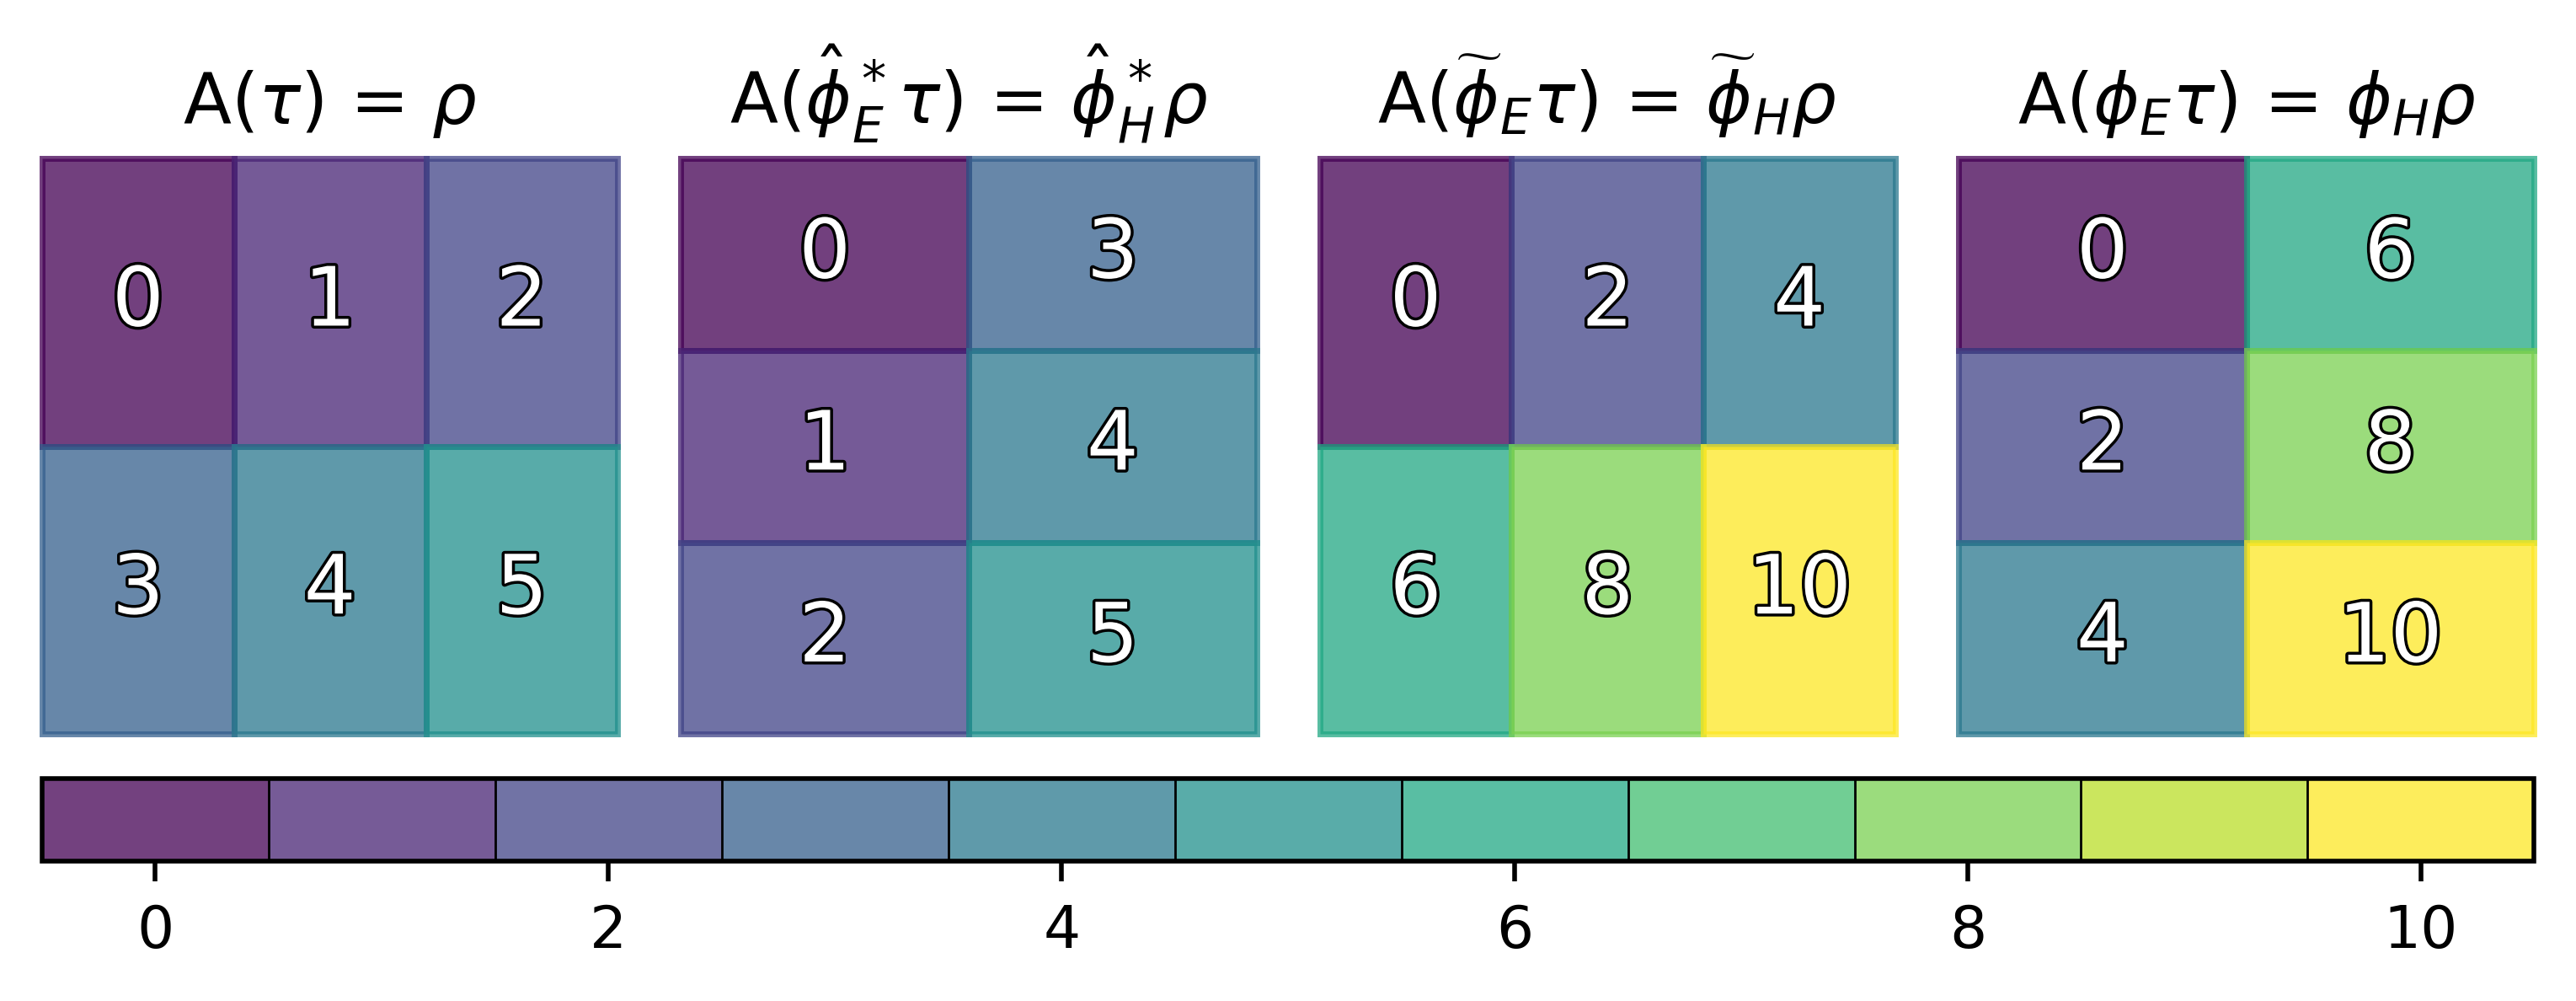
\includegraphics[width=1\columnwidth]{equivariance.png}
  \caption{This artist is equivariant because the input data and output graphic representation are transposed $\dfunch$, scaled $\dfunct$ and both transposed and scaled $\dfunc$ in the same manner.}
\end{figure}
For example, in \autoref{fig:artist:equivarance}, the measurable variable is color. This is a visual representation of the data shown in \autoref{fig:atct:phi}, and as such the equivariant transformations are an equivalent transposition and scaling of the colors. This visualization is equivariant with respect to base space transformations, as defined in \autoref{eq:atct:equivarance:verify:base}, because the color values at the new position at the old position $measure_\dbasepoint^{\prime} = \measure_{\dbasepoint}$. This visualization is also equivariant with respect to fiber wise transformations, as defined in \autoref{eq:atct:equivarance:verify:fiber}, because the colors are consistently scaled in the same was the data. For example, the values that have become 2 and 4 in the $\dfunctc$ and $\dfunc$ panels are colored the same as the original 2 and 4 values in the first panel. The equivariance in this visualization is composable, as shown in the colors being both transposed and scaled correctly in the $\dfunc$ panel.

\subsection{Composing Artists}\label{sec:artist:operators}
A common use of category theory in software engineering is the specification of modular components \cite{wielsManagementEvolvingSpecifications1998} such that we can build systems where the structure preserved by components is preserved in the composition of the components. This allows us to express that an artist that works on a dataset can be composed of artists that work on sub parts of that dataset. 
\begin{equation}
  \label{eq:artist:operator}
  \begin{tikzcd}[column sep=small]
      & \dfiberc^{a} \times_{\dfiberc^{c}} \dfiberc^{b} 
    \arrow[ld, "{\pi_{a\times b, a}}"', color=fiber] 
    \arrow[rd, "{\pi_{a\times b, b}}", color=fiber] & & 
    \dtotalc^{a} \oplus_{\dfiberc^{c}} \dtotalc^{b} 
    \arrow[ddd, "\pi"', color=total] \\
    \dfiberc^{a} 
    %\arrow[d, "\pi"', color=fiber] 
    \arrow[r, "{\pi_{a,c}}", color=fiber] 
    & \dfiberc^{c} & \dfiberc^{b} 
    %\arrow[d, "\pi", color=fiber] 
    \arrow[l, "{\pi_{b,c}}"', color=fiber] & \\
    \dbasec^{a} 
    \arrow[rd, "{\iota_{a, a+b}}"', color=base] 
    & \dbasec^{c} 
    \arrow[r, "{\iota_{c,b}}", color=base] 
    \arrow[l, "{\iota_{c,a}}"', color=base] 
    & \dbasec^{b} 
    \arrow[ld, "{\iota_{b, a+b}}", color=base] 
    &  \\
    & \dbasec^{a}\sqcup_{\dbasec^c}\dbasec^{b} & & 
    \dbasec^{a}\sqcup_{\dbasec^c}\dbasec^{b} 
    \arrow[uuu, "{\dsectionc^{a,b}}"', dashed, bend right, color=section]
  \end{tikzcd}
\end{equation}

\subsubsection{Addition: +}
\label{sec:artist:addition}
As illustrated in \autoref{eq:artist:operator}, data bundles can be combined by taking the disjoint  union of base spaces $\dbase^{a} \sqcup_{\dbase^c} \dbase^b$, where $\dbase^c$ is an overlap. When the fibers of each bundle are isomorphic $\dfiber^{a} \simeq \dfiber^{b}$, which we denote as $\dtotal$, this is analogous to adding more observations to a dataset. We propose an addition operator that states that an artist that takes in a dataset can be constructed using artists that take as inputs subsets of the dataset

\begin{equation*}
  \label{eq:artist:addition}
  \vartistc_{a+b}(\cgamma{\dbasec^{a} \sqcup_{\dbase^c} \dbasec^b}{\dtotalc}) \coloneqq \vartistc_{a}(\cgamma{\dbasec^{a}}{\dtotalc}) + \vartistc_{b}(\cgamma{\dbasec^{b}}{\dtotalc}) 
\end{equation*}
As introduce in $\autoref{eq:artist:hom_transport}$, the artist returns a function $\gsection$. We assume that the output space is a trivial bundle, which means that $\gsectionc \in Hom(\gbase, \gfiber)$ because the output specification is the same at each point $\gbase$. This allows us to make use of the hom set adjoint property\note{find citation}\
\begin{equation*}
  Hom(\gbase^{a} + \gbasec^b, \gfiber) = Hom(\gbase^{a}, \gfiber) + Hom(\gbase^b, \gfiber)
\end{equation*} 
to define an artist constructed via addition as consisting of two distinct graphic sections
\begin{equation}
  \label{eq:artist:plus:output}
  \gsectionc(\gbasepointc) \coloneqq \begin{cases} \gsectionc^{a}(\gbasepointc) & \gbasepointc \in \vindexprec(\dbasec^{a}) \\
    \gsectionc^{b}(\gbasepointc) & \gbasepointc \in \vindexprec(\dbasec^{b})
  \end{cases}
\end{equation}
that are evaluated only if the input graphic point is an the graphic area that graphic section acts on. 

One way to verify that these artists are composable is to check that the return the same graphic on points in the intersection $\dbase^{c}$.  Given $\dbasepointc_{a} \in \dbasec_{c} \subset \dbasec_{a}$ and $\dbasepointc_{b} \in \dbasec_{c} \subset \dbasec_{b}$, if $\dbasepointc_{a} = \dbasepointc_{b}$ then

\begin{equation}
  \label{eq:artist:plus:verify}
  \begin{split}
  &\vartistc_{a+b}(\dsectionc^{a+b}(\dbasepointc_{a})) \\ 
  & = \vartistc_{a}(\dsectionc^{a}(\dbasepointc_{a})) = \vartistc_{b}(\dsectionc^{b}(\dbasepointc_{b}))
  \end{split}
\end{equation}
 for all $\dbasepointc_{a}, \dbasepointc_{b} \in \dbasec_{a}\bigsqcup\limits_{\dbasec_{c}} \dbasec_{b}$  
 
 One example of an artist that is a sum of artists is a sphere drawer that draws different quadrants of a sphere $\vartist(\dsection) = \vartist_{1}(\dsection_{1}) + \vartist_{2}(\dsection_{2}) + \vartist_{3}(\dsection_{3}) \vartist_{4}(\dsection_{4})$. Given an input $\dbasepoint \in \dbase_4$ in the 4th quadrant, then the graphic section that would be executed is $\gsection_{4}$. If that point is also in the 3rd quadrant  $\dbasepoint \in \dbase_3$, then both artist outputs must return the same values $\gsection_{4}(\vindexprec(\dbasepoint)) = \gsection_{3}(\vindexprec(\dbasepoint))$. 


\subsubsection{Multiplication: $\times$}
\label{sec:artist:operator:multiplication}
As illustrated in \autoref{eq:artist:operator},  fibers that are a cartesian product of fiberspaces $\dfiber^{a} \times_{\dfiber^c} \dfiber^{b}$, where $\dfiber^c$ is any fiber that is present in both fibers, can be projected down into component fibers. In the trivial case where the base spaces are the same $\dbase^{a} = \dbase^{b} = \dbase$, this is equivalent to adding more fields to a dataset. 

\begin{equation*}
  \label{eq:artist:multiplication}
  \vartistc_{a \times b}(\cgamma{\dbase}{\dtotalc^{a\times b}}) \coloneqq \vartistc_{a}(\cgamma{\dbasec}{\dtotalc^{a}}) \times \vartistc_{b}(\cgamma{\dbasec}{\dtotalc^{b}}) 
\end{equation*}
which following from an adjoint property of homsets \note{find citation}
\begin{equation*}
  Hom(\gbase, \gfiber) \times Hom(\gbase, \gfiber) = Hom(\gbase, \gfiber\times \gfiber)
\end{equation*}
which means that the artists on the subsets of fibers can be defined 
\begin{equation}
  \gsectionc^{a \times b} = \{\gsectionc^{a}(\gbasepointc), \gsectionc^{b}(\gbasepointc)\}, \gbasepointc \in \vindexprec(\dbasec)
\end{equation} 
but that the signature of $\gsectionc^{a \times b}$ would be $\gbase \rightarrow \gfiber \times \gfiber$. Instead of having to special case the return type of artists that are compositions of multiple case, the hom adjoint \note{find cite} property
\begin{equation*}
  Hom(\gbase, \gfiber \times \gfiber) = Hom(\gbase+\gbase, \gfiber)
\end{equation*}
 means that multiplication can be considered as a special case of addition where $\dbase^{a} = \dbase^{b}$. While we discussed the trivial case in \autoref{sec:artist:addition}, there is no strict  requirement that $\dfiber^{a} = \dfiber^{b}$. 

One way to verify that these artists are composable is to check that they encode any shared fiber $\dfiber^{c}$ in the same way.

\begin{equation}
  \begin{split}
    &\extractmc(\vartistc_{a\times b}(\dsectionc^{a\times b}(\dbasepointc)))\restriction_{\dfiberc^{c}}\\ 
    &= 
    \extractmc(\vartistc_{a}(\dsectionc^{a}(\dbasepointc_{a})))\restriction_{\dfiberc^{c}} = \extractmc(\vartistc_{b}(\dsectionc^{b}(\dbasepointc_{b})))\restriction_{\dfiberc^{c}}
  \end{split}
\end{equation}

This expectation of using the same encoding for the same variable is a generalization of the concept of consistency checking of multiple view encodings discussed by Zening and Hullman \cite{hullmanKeeping2018}. This expectation can also be used to check that a multipart glyph is assembled correctly. For example, a box plot \cite{wickham40YearsBoxplots2011} typically consists of a rectangle, multiple lines, and scatter points; therefore a boxplot artist $\vartist_{boxplot} = \vartist_{rect} \times \vartist_{errors} \times \vartist_{line} \times \vartist_{points}$ must be constructed such that all the sub artists draw a graphic at or around the same x value. 

\begin{figure}[h!]
  \label{fig:artist:operator}
  \includegraphics*[width=1\columnwidth]{qcom.png}
  \caption{The circle-line glyph can either be considered as composed of two separate shapes, a circle and line, which each have their own graphic base spaces or as a single glyph which has an equivalent graphic base  $\gbase_{circle} \sqcup \gbase_{line} = \gbase_{circle-line}$ }
\end{figure}

The circle-line glyph in \autoref{fig:artist:operator} can be generated via a line plot and highlighted points in that plot, which is the addition case of two datasets with the same fields and different continuities. The same circle-line glyph can also be generated via the multiplication case as different fields of the same bundle. As mentioned in \autoref{sec:artist:operator:multiplication}, multiplication is implemented as addition of two copies of a base space. Although we have been discussing the trivial cases of adding observations or adding fields, this merging of artists in datasets can be generalized:
\begin{equation}
  \vartistc(\cgamma{\mathop{\sqcup}_{i} \dbasec^{i}}{\mathop{\oplus}_{i}\dtotalc^{i}}) \coloneqq \sum_{i}
  \vartistc_{i}(\cgamma{\dbasec^{i}}{\dtotalc^{i}}) 
\end{equation} 

As shown in \autoref{eq:artist:operator}, bundles over a union of base spaces can be joined as a product of the fibers. This allows us to consider all the data inputs in a complex visualization as a combined input, where some sections evaluate to null in fields for which there are no values for that point in the combined base space $\dbasepoint \in \mathop{\sqcup}_{i} \dbase^{i}$ The combined construction of the data is a method for expressing what each data input has in common with another data input-for example the data for labeling tick marks or legends- 
and therefore which commonalities need to be preserved in the artists that act on these inputs. 

\section{Construction}
\label{sec:construction}
\begin{figure}[h!]
  \label{fig:construction:flow}
  \includegraphics*[width=1\columnwidth]{path_of_q.png}
  \caption{One method of constructing the artist is by formulating the artist as having two stages: (1) encoding functions $\vchannelc$ that convert different parts of the input into measurable visual components, such as color or position; (2) compositing functions $\vmarkc$ that assemble the measurable visual components into a visual element generating function. In this construction, we propose an intermediate visual bundle $\vtotalc$ that encodes the space of possible visual encodings.}
\end{figure}
We propose that one way of constructing artist functions is to separate generating a visualization, as shown in \autoref{fig:construction:flow}, is into an equivariant continuity preserving encoding stage $\vchannelc$ and a equivariant continuity preserving compositing stage $\vmarkc$. In the \textcolor{artist}{encoding} stage $\vchannelc$, a data bundle is treated as separable fields and each field is mapped to a measurable visual variable. In the encoding stage, the expected visual mappings $\equivb$ can be implemented inside the library. Factoring out the encoding stage leaves the \textcolor{artist}{compositing} stage $\vmarkc$ responsible for faithfully translating those measurable visual components into a visual element.  

\subsection{Measurable Visual Components}
\label{sec:construction:vtotal}
As shown in \autoref{fig:construction:flow}, we propose an intermediate visual fiber bundle 
\begin{equation}
  \vfiberc \hookrightarrow \vtotalc \xrightarrow{\pi} \dbasec
\end{equation}
where the space of possible visual encodings is the fiber space $\vfiber$. The space of visual sections which return visual encoding specifications is 
\begin{equation}
\cgamma{\opensetc}{\vtotalc\restriction_{\opensetc}} \coloneqq \big\{\vsectionc: \opensetc\rightarrow \vtotalc\restriction_{\opensetc} \; \bigm{\vert} \pi(\vsectionc(\dbasepointc)) = \dbasepointc\;for\, all\; \dbasepointc \in \opensetc \big\} 
\end{equation}
As shown in \autoref{eq:artist:inout:diagram},  measurable visual components are defined as having the same continuity as the data $\dbase$. This means that every data record $\dsection(\dbasepoint)$ has a corresponding visual section such that $\pi(\dsection(\dbasepoint)) = \pi(\vsection(\dbasepoint))$. 

Although the bundle $\vtotal$ is structurally equivalent to the bundle $\dtotal$, its existence allows for separating the data that is input into the artist $\dsection$ from the data internal to the artist $\vsection$. This allows a visualization library to define a visual bundle space $\vtotalc$ the holds the internal representation standard for measurable visual components. For example, a visualization library could define a visual color fiber as an RGBA tuple $\vfiber_{color} = \mathbb{R}^{3} \times [0,1]$. This would then set the expectation that arbitrary color encoding functions would need to return an RGBA tuple for the library to recognize the encoding as a color. 

\subsection{Defining Maps Between Spaces $\vindex$}
In \autoref{sec:atct:sheaves}, the functors $\vindex, \vindexpull, \vindexpushc$ are introduced to describe the expected relationship between screen and data base spaces. In the construction of the artist, the functor $\vindex$ is defined such that the data base space \dbase\ is a deformation retraction\cite{nlab:deformation_retract} of the graphic space $\gbase$. This means that there is a continuous surjective mapping from every point $\dbasepoint\in\dbase$ to a point $\dbasepoint \in dbase$. To simplify matters, in this paper, we construct the graphic space as a constant multiple of the base space such that 
\begin{equation}
  \underbrace{\dbasec\times[0,1]^{n}}_{\gbasec} \textcolor{functor}{\xmapsto{\hspace{1em}\vindexc\hspace{1em}}} \dbasec
\end{equation}
where n is a thickening of the graphic base space $\gbase$ to account for the dimensionality of the output space
\begin{equation*}
  n = \begin{cases}
    dim(\gbase) - dim(\dbase) & dim(\dbase)<dim(\gbase)\\
  0 & otherwise
  \end{cases}
\end{equation*}
because the data dimensionality $\dbase$ may be too small for a graphic representation.

\begin{figure}[h!]
  \label{fig:construction:xi}
  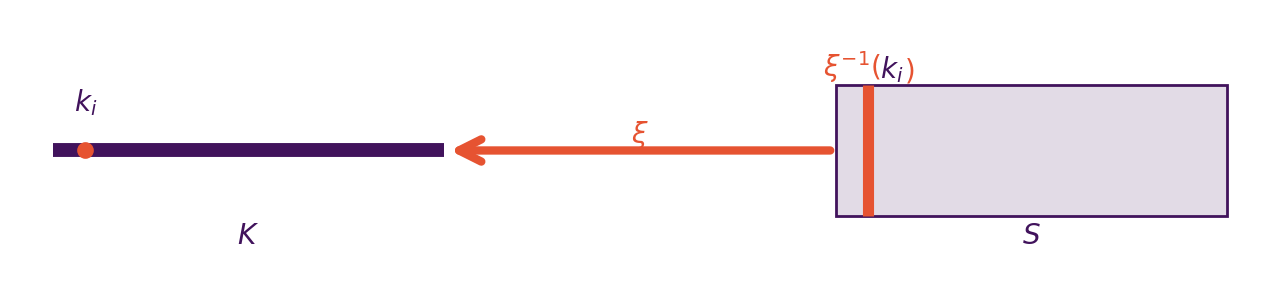
\includegraphics[width=1\columnwidth]{deform_retract.png}
  \caption{The graphic base space $\gbase$ is collapsable to the line $\dbase$ such that every band $(\dbasepoint_i, [0,1])$ on $\gbase$ maps to corresponding point $\dbasepoint_i \in \dbase$ and the band $[0,1]$ determines which pixels are filled in to generate the shape of the line.\note{maybe put in a phantom line plot in s}}
\end{figure}
For example, as shown in \autoref{fig:construction:xi}, a line is 1D but is a 2D glyph on a screen; therefore the graphic space $\gbase$ is constructed by multiplying the base space $\dbase$ with an interval $[0,1]$. Because $\gbase$ is collapsible into $\dbase$, every band $(\dbasepoint_i, [0,1])$ corresponds to a point in the base space $\dbasepoint_i \in \dbase$. The first coordinate $\alpha=\dbasepoint_i$ provides a lookup to retrieve the associated visual variables. The second coordinate, which is a point in the interval $\beta=[0,1]$. Together they are a point $\gbasepoint=(\alpha,\beta) \in gbase$ in the graphic base space. This point $\gbasepoint$ is the input into the graphic section $\gsection(\gbasepoint)$ that is used to determine which pixels are colored, which in turn determines the thickness, texture, and color of the line. 


\subsection{Encode Data as Measurable Components}
\label{sec:construction:nu}
As introduced in \autoref{fig:construction:flow}, the encoding function $\vchannel$ is a map from data sections to graphic sections
\begin{equation}
\nu: \cgamma{\dbasec}{\dtotalc} \rightarrow \cgamma{\dbasec}{\vtotalc}
\end{equation}
such that the sections project to the same point on the base space $\pi(\dtotal) = \pi(\vchannel(\dtotal))$. A consequence of this property is that $\vchannelc$ can be constructed as a pointwise transformation such that  
\begin{equation}
  \label{eq:constrution:nu}
  \vchannelc: \dfiberc_{\dbasepointc} \rightarrow \vfiberc_{\dbasepoint}
\end{equation}
which means that means that a point in a single data fiber $\delement \in \dfiber_{\dbasepointc}$ can be mapped into a corresponding point in a visual fiber $\velement \in \vfiber_{\dbasepointc}$. This means that an encoding function $\vchannel$ can convert a single record and may not need the whole dataset. 

The difference between $\dtotal$ and $\vtotal$ are semantic rather than structural; they are both maps from the topological space \dbase\ to sets of functions that return records of values. This means any $\vtotal$ can be redefined as $\dtotal$, 
\begin{equation}
  \label{eq:construction:nu:fabrication}
  \begin{tikzcd}[col sep=Huge]
    \dfiberc_{\dbasepointc} 
    \arrow[rr, "\vchannelc", color=artist] 
    \arrow[rrrr, "\vchannelc^{\prime\prime}", dashed, bend right, color=artist] &  & 
    \vfiberc_{\dbasepointc}\coloneqq{\dfiberc_{\dbasepointc}^{\prime}} 
    \arrow[rr, "\vchannelc^{\prime}", color=artist] &  & 
    \vfiberc^{\prime}_{\dbasepointc}
  \end{tikzcd}
\end{equation}
which means that, as shown in \autoref{eq:construction:nu:fabrication}, any collection of $\vchannel$ functions can be composed such that they are equivalent to a $\vchannel$ that directly converts the input to the output. This means that a developer has the flexibility to implement either the direct convertor or the building block version (or both) depending on other library concerns. As with artists, $\vchannel$ are maps of sections such that the composition operators defined in \autoref{sec:artist:composition} can also act on transformers $\vchannel$, meaning that encoders can be added and multiplied. 

\subsubsection{Encoder Verification}
\label{sec:construction:nu:verification}
A  motivation for constructing an artist with an encoder stage $\vchannel$ is so that the conversion from data to measurable component can be tested separately from the assembly of components into a glyph. 
\begin{equation}
  \label{eq:construction:nu:validate}
  \begin{tikzcd}[column sep=4em]
    {\dfiberc_{\dbasepointc}^{a}} \times {\dfiberc_{\dbasepointc}^{b}} 
    \arrow[d, "\pi_a"', color=fiber] 
    \arrow[r, "\vchannelc_{ab}", color=artist] 
    \arrow[rr, "\equivc_{ab}", bend left, color=monoid]  & 
    {\vfiberc_{\dbasepointc}^{a}} \times {\vfiberc_{\dbasepointc}^{b}} 
    \arrow[d, "\pi_a", color=fiber] & 
    \measurec_{\dbasepointc}^{ab} 
    \arrow[d, "\measurec\restriction_a", color=set] \\
    \dfiberc_{\dbasepointc}^a 
    \arrow[r, "\vchannelc_{a}", dashed, color=artist] & 
    \vfiberc_{\dbasepointc}^a 
    \arrow[r, "\simeq", dotted]  & 
    \measurec_{\dbasepointc}^a   \\
    {\dfiberc_{\dbasepointc}^{a}} \times {\dfiberc_{\dbasepointc}^{c}} 
    \arrow[u, "\pi_a", color=fiber] 
    \arrow[r, "\vchannelc_{ac}", color=artist] 
    \arrow[rr, "\equivc_{ac}", bend right, color=monoid] & 
    {\vfiberc_{\dbasepointc}^{a}} \times {\vfiberc_{\dbasepointc}^{c}} 
    \arrow[u, "\pi_a"', color=fiber] & 
    \measurec_{\dbasepointc}^{ac} 
    \arrow[u, "\measurec\restriction_a"', color=set]            
    \end{tikzcd}
\end{equation}
As shown in \autoref{eq:construction:nu:validate}, an encoder is considered valid if there is an ismorphism between the actual outputted visual component and the expected measurable component encoding. An encoder is consistent if it encodes the same field in the same way even if coming from different data sources. 

An encoding function $\vchannelc$ is equivariant if the change in data, as defined in \autoref{sec:atct:sheaves:measurments}, and change in visual components are equivariant. Since $\dtotal$ and $\vtotal$ are over the same base space and are pointwise, the base space change $\dfunch_{\dtotal}$ applies to both sides of the equation 
\begin{equation}
  \vchannelc(\dsectionc_{\dtotalc}(\dfunchc_{\dbasec}(\dbasepointc^{\prime}))) = \vsectionc(\dfunchc_{\dbasec}(\dbasepointc^{\prime}))
\end{equation}
and therefore there should not be a change in encoding. On the other hand, a change in the data values $\dfunct_{\dtotal}$ must have an equivalent change in visual components
\begin{equation}
  \dfunctc_{\vtotalc} \vchannelc(\dsectionc(\dbasepoint)) = \vchannelc(\dfunctc_{\dtotalc}(\dsectionc(\dbasepointc)))
\end{equation}
The change in visual components $\dfunct_{\vtotal}$ is dependent both on $\dfunct_{\dtotal}$ and the choice of visual encoding. As mentioned in \autoref{sec:related-work:equivariance}, this is why Bertin and many others since have advocated choosing an encoding that has a structure that matches the data structure\cite{bertinSemiologyGraphicsDiagrams2011a}. For example choosing a quantative colormap to encode quantative data if the $\dfunctc$ operation is scaling, as in \autoref{fig:artist:equivariance}.


\subsection{Composite Measurable Components Into Visual Elements}
As shown in \autoref{fig:construction:flow}, the compositor function $\vmarkc$ transforms the measurable components into properties of a visual element. The compositing function $\vmarkc$ transforms the sections of visual elements $\vsectionc$ into sections of graphics $\gsectionc$.
\begin{equation}
  \vmarkc: \cgamma{\dbasec}{\vtotalc} \rightarrow \cgamma{\gbasec}{\gtotalc}
\end{equation}
The compositing function is map from sheaves over $\dbase$ to sheaves over $\gbase$. This is because, as described in \autoref{fig:construction:xi}, the graphic section must be evaluated on all points in the graphic space to generate the visual element corresponding to a data record at a single point $\vartist(\dsection(\dbasepoint)) = \gsection(\vindexpre(\dbasepoint))$. 

Since encoder functions are infinitely composable, as described in \autoref{eq:construction:nu:fabrication}, a new compositor function $\vmarkc$ can be constructed by precomposing $\vchannelc$ functions with the existing $\vmarkc$.

\begin{equation}
  \label{eq:construction:q:fabrication}
  \begin{tikzcd}
      \cgamma{\dbasec}{\vtotalc} 
      \arrow[rr, "\vchannel", color=artist] 
      \arrow[rrrr, "\vmarkc^{\prime}", bend right, color=artist, dashed] &  & \cgamma{\dbasec}{\vtotalc^{\prime}} 
      \arrow[rr, "\vmarkc", color=artist] &  & \cgamma{\gbasec}{\gtotalc}
      \end{tikzcd} 
\end{equation}
The composition in \autoref{eq:construction:q:fabrication} means that different measurable components can yield the same visual elements. 

\begin{figure}[h!]
  \label{fig:construction:q}
  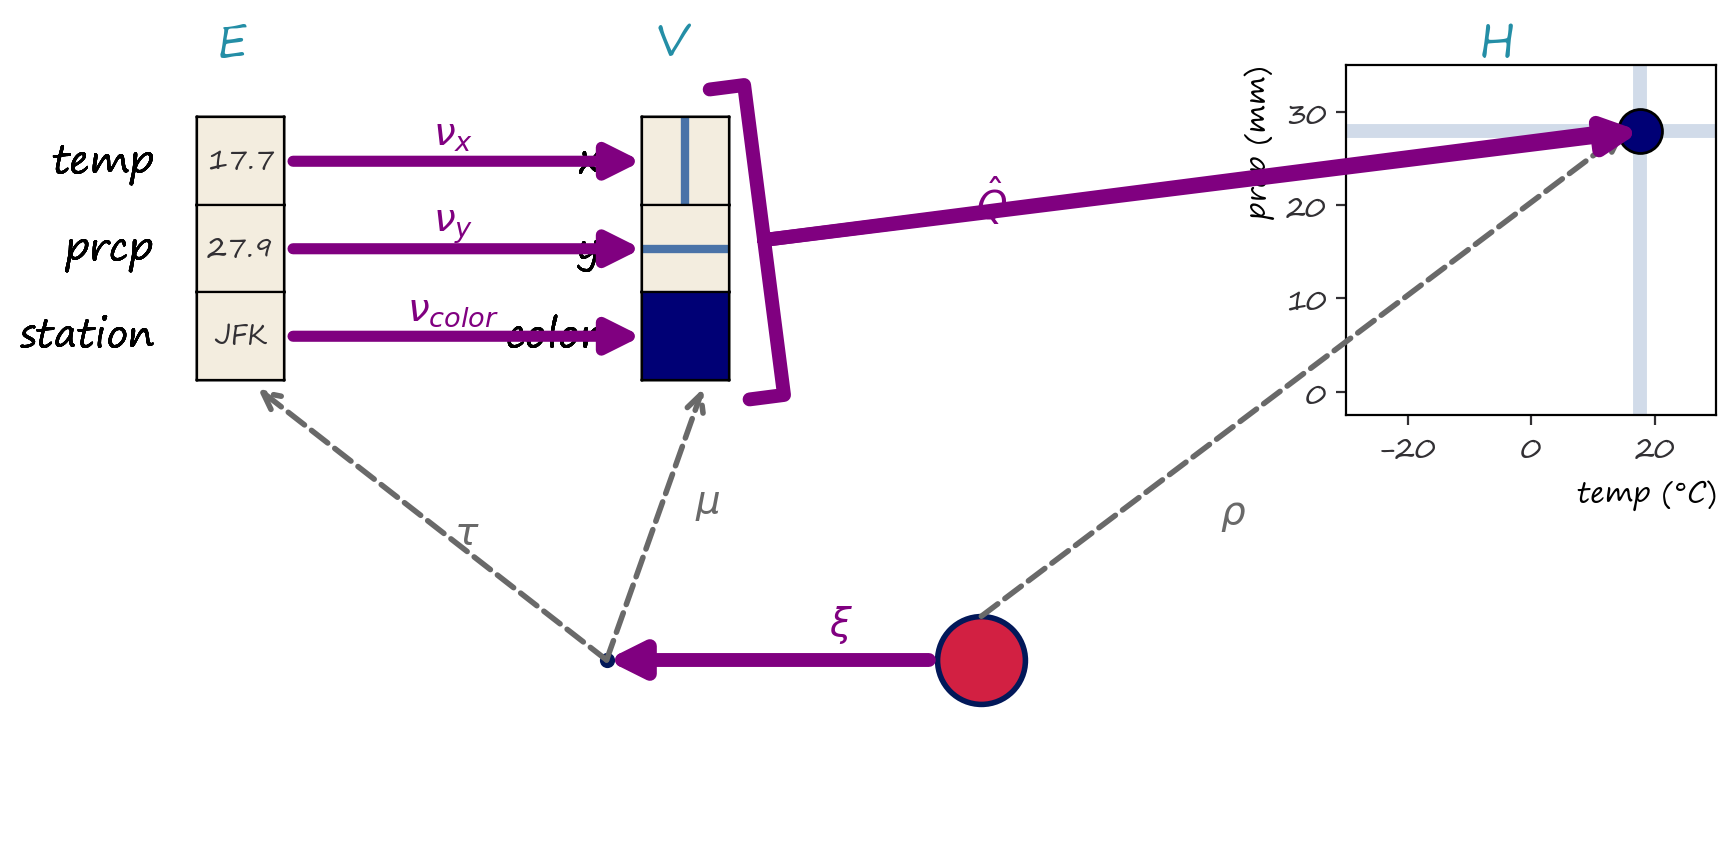
\includegraphics[width=1\columnwidth]{q.png}
  \caption{This simple $\vmarkc$ assembles a circular visual element that is the color specified in $\vsection(\dbasepoint)$ and is at the intersection specified in $\vsection(\dbasepoint)$}
\end{figure}
As shown in \autoref{fig:construction:q}, a set of  $\vchannel$ functions individually convert the values in the data record to visual components. Then the $\vmarkc$ function combines these visual encodings to produce a graphic section \gsection. When this section is evaluated on the graphic space associated with the data $\gsection(\vindexpre(\dbasepoint))$, it produces a blue circular marker at the intersection of the x and y positions listed in \vsection. The composition rule in \autoref{eq:construction:q:fabrication} means that developers can implement $\vmarkc$ as drawing circles or can implement a $\vmarkc$ that draws arbitrary shapes, and then provide different $\vchannelc$ adapters, such as one that specifies that the shape is a circle. 

\subsubsection{Compositor Verification}
\label{sec:construction:q:verification}
An advantage of factoring out encoding and verification, as discussed in \autoref{sec:construction:nu:verification}, is that the responsibility of the compositor can be scoped to translating measurable components into visual elements. 
\begin{equation}
  \label{eq:construction:q:validate}
  \begin{tikzcd}[row sep=huge]
    \cgamma{\dbasec}{\vtotalc^{a}\times \vtotalc^{b}}  
    \arrow[rr, "\vmarkc_{ab}", color=artist] 
    \arrow[d, "\pi_a"', color=total] &  &  \imartistsub{ab}{\gbasec}{\gtotalc} 
    \arrow[d, "\measurec\restriction_a \circ \extractmc_{ab}", color=monoid]  \\
   \cgamma{\dbasec}{\vtotalc^{a}} 
   \arrow[rr, "\simeq", dotted] &  & 
   {\textcolor{set}{Hom}(\dbasec, \measurec^{a})}  \\
    \cgamma{\dbasec}{\vtotalc^{a}\times \vtotalc^{c}}  
    \arrow[rr, "\vmarkc_{ac}", color=artist] 
    \arrow[u, "\pi_a", color=total]  &  &  \imartistsub{ac}{\gbasec}{\gtotalc} 
    \arrow[u, "\measurec\restriction_a \circ \extractmc_{ac}"', color=monoid]
   \end{tikzcd}
\end{equation}
As illustrated in \autoref{eq:construction:q:validate}, a compositor is valid if there is an isomorphism between the actual outputted measured visual component and the expected measurable component that is the input. One way of verifying that a compositor is consistent is by verifying that it passes through one encoding even while changing others. For example, when $\vmark_{ab}=\vmark_{ac}$ then the output should differ in the same measurable components as $\vsectionc_{ab}$ and $\vsection_{ac}$. 

A compositor function \vmark\ is equivariant if the renderer output changes in a way equivariant to the data transformation defined in \autoref{sec:atct:sheaves:measurments}. This means that a change in base space $\dfunch_{\dtotalc}$ should have an equivalent change in visual element base space. This means that there should be no change in visual measurement
\begin{equation}
  \label{eq:construction:q:verification:base}
  \vsectionc(\dfunchc_{\dbasec}(\dbasepointc^{\prime})) = \extractmc(\vmarkc(\vsectionc)(\dfunch_{\dbasec}(\vindexpre^{\dbasepointc}))) = \measurec_{\dbasepointc}
\end{equation}
As discussed in \autoref{fig:artist:equivariance}, the change in base space may induce a change in locations of measurements relative to each other in the output; this can be verified via checking that all the measurements have not changed relative to the original positions $\measurec_{\dbasepoint} = \measurec_{\dbasepointc^{\prime}}$ and through separate measurable variables that encode holistic data properties, such as orientation or origin. 

The compositor function is also expected to be equivariant with respect to changes in data and measurable components
\begin{equation}
  \label{eq:construnction:nu:verify:base}
  \dfunctc_{\vtotalc}(\vsectionc(\dbasepointc)) = \dfunctc_{\gtotalc}(\vmarkc(\vsectionc(\dbasepointc)))  
\end{equation}
which means that any change to a measurable component input must have a measurably equivalent change in the output. As illustrated in \autoref{fig:artist:equivariance}, the compositor $\vmarkc$ is expected to assemble the measurable components such that base space changes, for example transposition, are reflected in the output; faithfully pass through equivariant measurable components, such as scaled colors; and ensure that both types of transformations, here scaling and transposition, are present in the final glyph.  


\subsection{Constructing the Artist: $\vartistc=\vmarkc\circ\vchannelc$}

As shown in \autoref{eq:atct:sheaves:homset}, if a sheaf is equipped with transport functors, then the functions between sheaves over one space are isomorphic to functions between sheave over the other space. This property, allows us to specify the transformation from data to graphic space in data or graphic space or a combination, as listed in \autoref{eq:artist:hom_transport}, such that the following diagram commutes:
\begin{equation}
  \label{eq:construction:artist:path}
\begin{tikzcd}[row sep=2.5em, column sep=1.5em]
  \cgamma{\dbasec}{\dtotalc} 
  \arrow[rr, "\vchannelc^{\dbasec}", color=artist] 
  \arrow[rrrr, "\vartistc^{\dbasec}", bend left, color=artist] 
  \arrow[dd, "\vindexpullc"', color=functor] 
  \arrow[rrrrdd, "\vartistc", color=artist, pos=.2] &  & 
  \cgamma{\dbasec}{\vtotalc} 
  \arrow[rrdd, "\vmarkc", color=artist] 
  \arrow[rr, "\vmarkc^{\dbasec}", color=artist] 
  \arrow[dd, "\vindexpullc", color=functor, pos=.2] &  & \imartist{\dbasec}{\vindexpushc\gtotalc}  \\
   & & & & \\
  \cgamma{\gbasec}{\vindexpullc\dtotalc} 
  \arrow[rr, "\vchannelc^{\gbasec}", color=artist] 
  \arrow[rrrr, "\vartistc^{\gbasec}", bend right, color=artist] & & 
  \cgamma{\gbasec}{\vindexpullc\vtotalc} 
  \arrow[rr, "\vmarkc^{\gbasec}", color=artist] &  & 
  \imartist{\gbasec}{\gtotalc} 
  \arrow[uu, "\vindexpushc"', color=functor]
\end{tikzcd}  
\end{equation}
The diagram in \autoref{eq:construction:artist:path} illustrates how a developer can connect transformations over data space, denoted with a subset $\dbase$, with transformations over graphic space $\gbase$, using $\vindexpushc$ and $\vindexpullc$ adaptors. This allows developers to for example connect transformers that transform data on a line to a color in dataspace, but build a line compositing function that dynamically resamples what is on screen in graphic space.

\section{Discussion: Implementing The Math}
\label{sec:discussion}
The framework specified in \autoref{sec:artist} and \autoref{sec:construction} describes how to build structure preserving visualization components, but it is left to the library developer to follow these guidelines when building and reusing components. 
In this section, we introduce a toy example of building an artist out of the components introduced in \autoref{sec:construction} to illustrate how components that adhere to these specifications are maintainable, extendible, scalable, and support concurrency. Specially, we introduce artists for building different types of bar graphs because it is a visualization type that allows us to demonstrate composability and multivariate data encoding. We build our visualization components by extending the Python visualization library Matplotlib's artist\footnote{Matplotlib artists are our artist's namesake}\cite{hunterMatplotlib2DGraphics2007,hunterArchitectureOpenSource} to show that components using this model can be incorporated into existing visualization libraries iteratively. While the architecture specified in \autoref{sec:construction} can be implemented fully functionally, we make use of objects to keep track of parameters passed into artists. In this toy example, the small composable components allow for more easily verifying that each component does its transformation correctly before assembling them into larger systems.  


\begin{table}[h!]
  \centering
\begin{tabular}{|lcl|}
  \hline \\
   fruit &  calories &  juice \\
  \hline\\
    apple &        95 &   True \\ 
   orange &        67 &   True \\ 
  lemon &        17 &  False \\ 
      lime &        20 &  False \\
  \hline
\end{tabular}
\label{tab:discussion:data}
\end{table}
We construct a toy dataset with a discrete $\dbase$ of 4 points and a fiber space of $\dfiber=\{apple,\, orange,\, lemon\}\times \mathbb{Z}^{+} \times \{\texttt{True}, \texttt{False}\}$. We thinly wrap \autoref{tab:discussion:data} in an object so that the common data interface function is that $\tau = \ttexttt{DataContainerObject.query}$. 
\begin{minted}{python}
  class FruitFrameWrapper:
    def query(self, data_bounds, sampling_rate):
      # local sections are a list of
      # {field: local_batch_of_values}
      return local_sections
\end{minted}

This interface provides a uniform way of accessing subsets of the data, which are local sections. The motivation for a common data interface is that it would allow the artist to talk to different common python data containers, such as numpy\cite{harris2020array}, pandas\cite{jeff_reback_2020_3715232}, xarray \cite{hoyer2017xarray}, and networkx\cite{HagbergExploringNetwork2008}. Currently, data stored in these containers must be unpacked and converted into arrays and matrices in ways that either destroy or recreate the structure encoded in the container. For example a pandas data frame must be unpacked into its columns before it is sent into most artists and continuity is implicit in the columns being the same length rather than a tracked base space $\dbase$.

Because it is more efficient to work with the data in column order, we often treat the data as a collection of single fiber bundles. This is equivalent to the total bundle, as shown in \autoref{eq:artist:operator}. To encode the values in the dataset, we enforce equivariance by writing $\vchannel$ encoders that match the structure of the fields in the dataset. For example, the fruit column is a nominal measurement scale. Therefore we implement a position encoder that respects permutation $\dfunch$ transformations. The most simple form of this $\vchannel$ is a python dictionary that returns an integer position, because Matplotlib's internal parameter space expects a numerical position type. 
\begin{minted}{python}
  def position_encoder(val):
    return {'apple': 0, 'orange': 2, 'lemon': 4, 'lime': 6}[val]
\end{minted}
As mentioned in \autoref{eq:construction:nu:fabrication}, the encoders can be composed up. For example, the compositor $\vchannel$ may need the position to be converted to screen coordinates. Here the screen coordinate $\vchannel$ is a method of a Matplotlib axes object; a Matplotlib axes is akin to a container artist that holds all information about the sub artists plotted within it. 
\begin{minted}{python}
def composite_x_transform(ax, nu):
    return lambda x: ax.transData.transform(
            (position_encoder(x), 0))[0]
\end{minted}
This encoder returns a function that is \texttt{transData.transform} $\vchannel_{transData}$ composed with the position encoder $\vchannel_{position}$ and takes as input a record to be encoded. As with the position encoder, the transData encoder respects permutation transforms because it returns reals; therefore the composite encoder respects permutation transforms. In this model, developers implement $\vchannel$ encoders that are explicit about which $\dfunc_{\vtotal}$ they support. Writing semantically correct encoders is also the responsibility of the developer and is not addressed in the model. For example \mintinline{python}{fruit_encoder = lamda x: {'apple': green, 'orange':'yellow', 'lemon':'red', 'lime':'orange'}} is a valid color encoding with respect to permutation, but none of those colors are intuitive to the data. It is therefore left to the user, or domain specific library developer, to choose $\vchannel$ encoders that are appropriate for their data.

After converting each record into an intermediate visual component $\vsection$, the set of visual records is passed into $\vmarkc$. Here the $\vmarkc$ includes one last encoder, as illustrated in \autoref{eq:construction:q:fabrication}, that assembles the independent visual components into a rectangle. This $\vchannel$ is inside the $\vmarkc$ to hide that library preferred format from the user. It is called \texttt{qhat} to indicate that this is the $\vartist^{\dbase}$ path in \autoref{eq:construction:artist:path}.  This means that the parameters are constructed in data space $\dbase$ and this function returns a pushed forward $\vindexpush\gsection$. 

\begin{minted}{python}
   def qhat(position, width, length, floor, facecolor, edgecolor, linewidth, linestyle): 
        box = box_nu(position, width, length, floor)
        def fake_draw(render, transform=mtransforms.IdentityTransform()):
            for (bx, fc, ec, lw, ls) in zip(box, facecolor, edgecolor, linewidth, linestyle):
                gc = render.new_gc()
                gc.set_foreground((ec.r, ec.g, ec.b, ec.a))
                gc.set_dashes(*ls)
                gc.set_linewidth(lw)
                render.draw_path(gc=gc, path=bx, transform=transform, rgbFace=(fc.r, fc.g, fc.b, fc.a))
        return fake_draw
\end{minted}
The function \texttt{fake\_draw} is the analog of $\vindexpush\gsection$. This function builds the rendering spec through the renderer API, and this curried function is returned. The transform here is required for the code to run, but is set to identity meaning that this function directly uses the output of the position encoders. The curried $\texttt{fake\_draw} \approx \vindexpush \gsection$ is evaluated using a renderer object. In our model, as shown in \autoref{eq:artist:inout:diagram}, the renderer is supposed to take $\gsection$ as input such that $renderer(\gsection) = visualization$, but here that would require an out of scope patching of the Matplotlib render objects. 

The $\vchannel$ and $\vmark$ are wrapped in a container object that stores the $\vartist = \vmark \circ \vchannel$ composition and a method for computing the $\vsectionc$.
\begin{minted}{python}
  class Bar: 
    def compose_with_nu(self, pfield, ffield, 
          nu, nu_inv:):
        # returns a new copy of the Bar artist 
        # with the additional nu that converts 
        # from a data (F) field value to a 
        # visual (P) field value
        return new

    def nu(self, tau_local): #draw
       # uses the stored nus to convert data
       # stored nus have F->P field info
      return mus
    
    @staticmethod
    def qhat(position, width, length, floor, facecolor, edgecolor, linewidth, linestyle):
       
        return fake_draw
\end{minted}

This artist is then passed along to a shim artist that makes it compatible with existing Matplotlib objects
\begin{minted}{python}
class GenericArtist(martist.Artist):
    def __init__(self, artist:TopologicalArtist):
        super().__init__()
        self.artist = artist
        
    def compose_with_tau(self, section):
        self.section = section

    def draw(self, renderer, bounds, rate):
        for tau_local in self.section.query(bounds, rate): 
            mu = self.artist.nu(tau_local)
            rho = self.artist.qhat(**mu)
            output = rho(renderer)
\end{minted}
As shown in the \texttt{draw} method, generating a graphic section $\gsection$ is implemented as the composition of $\texttt{qhat} \approx \vmark$ and $\texttt{nu} \approx \vchannel$ applied to a local section of the sheaf $\textttt{self.section.query} \approx \desection^{i}$ such  $\texttt{draw} \approx \vmarkc\circ\vchannelc\circ\dsectionc  = \vartistc\circ \dsectionc$. The $\vchannel$ and $\vmark$ functions shown here are written such that they can generate a visual element given a local section $\dsection\restriction_{\dbase^{i}}$ which can be as little or large as needed. This flexibility is a prerequisite for building scalable and streaming visualizations that may not have access to all the data. 

\begin{figure}[h!]
  \centering
  \subfloat[]{
    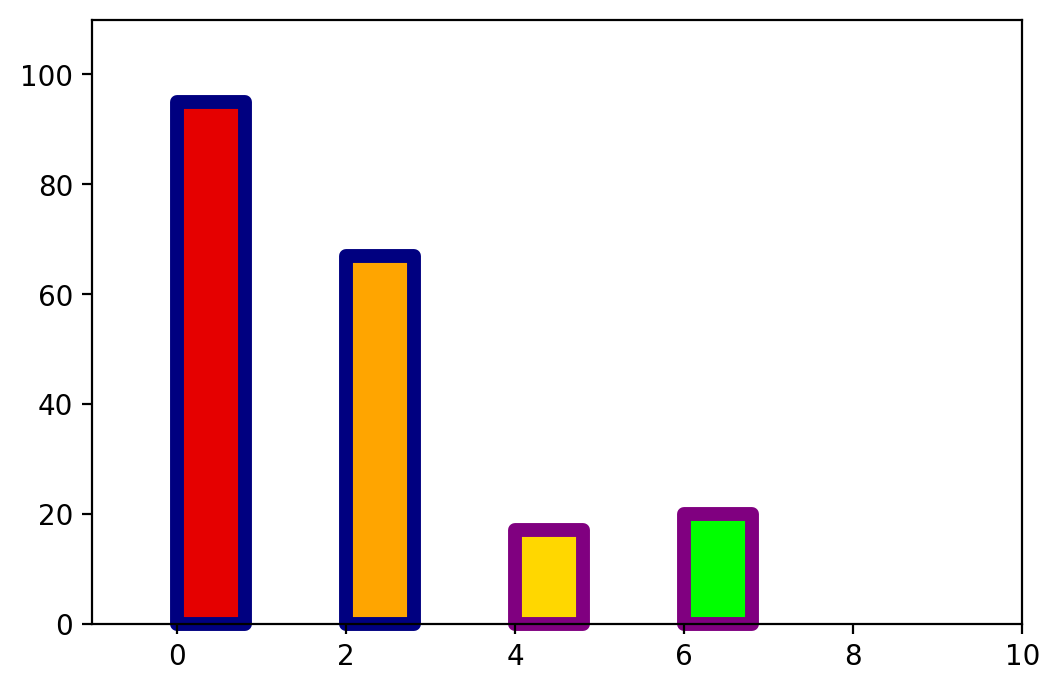
\includegraphics[width=.45\columnwidth]{bar.png}
  \label{fig:discussion:vbar}}
  \subfloat[]{
    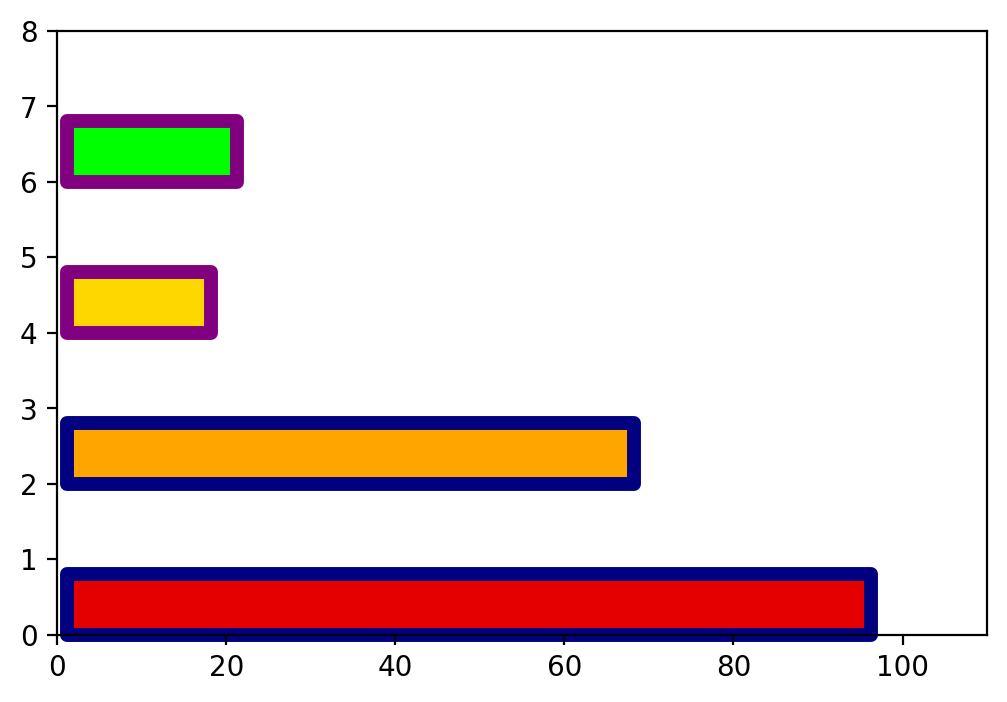
\includegraphics[width=.45\columnwidth]{barh.png}
  \label{fig:discussion:hbar}
  }
  \label{fig:discussion:bar}
\end{figure}

The \texttt{GenericArtist} is a a standard Matplotlib object; therefore it can be hooked into the Matplotlib draw tree to produce the vertical bar chart in \autoref{fig:discussion:vbar}. Using the Matplotlib artist framework means this new artist can be composed with existing artists, such as the ones that draw the axes and ticks. 

One of the advantages of this model is that it allows for succinctly expressing the difference between two very similar visualizations, such as \autoref{fig:discussion:vbar} and \autoref{fig:discussion:hbar}. In this model, the horizontal bar is implemented as a composition of a $\vchannel$ that renames fields in $\vsection_{barh}$ and the $\vmark$ implementation for the horizontal bar.
\begin{minted}{python}
def qhat(length, width, position, floor, facecolor, edgecolor, linewidth, linestyle):
  return Bar.qhat(**BarH.bar_nu(length, width, position, floor, facecolor, edgecolor, linewidth, linestyle))
\end{minted}
This composition is equivalent to $\vmark_{barh} = \vmark_{bar} \circ \vchannel_{vtoh}$, which is an example of \autoref{eq:construction:q:fabrication}. These functions can be further added together, as described in \autoref{sec:artist:operators} to build more complex visualizations. 

The example in this section is intentionally trivial to illustrate that the math to code translation is fairly straightforward and results in fairly self contained composable functions. Further research could investigate building new systems using this model, specifically libraries for visualizing domain specific structured data and domain specific artists. More research could also explore applying this model to visualizing high dimensional data, particularly building artists that take as input distributed data and artists that are concurrent. Developing complex systems could also be an avenue to codify how interactive techniques are expressed in this framework.


\section{Conclusion}
The toy example presented in \autoref{sec:discussion} demonstrates that it is relatively straightforward to build working visualization library components using the construction described in \autoref{sec:construction}. Since these components are defined with single record inputs, the can be implemented such that they are concurrent. The cost of building a new function using these components is sometimes as small as renaming fields, meaning the new feature is relatively easy to maintain. These new components are also a lower maintenance burden because, by definition, they are designed in conjunction with tests that verify that they are equivariant.  
These new components are also compatible with the existing library architecture, allowing for a slow iterative transition to components built using this framework. 
The framework introduced in this paper is a marriage of the ways the graphic and data visualization communities approach visualization. The graphic community prioritizes \note{?} how input is translated to output, which is encapsulated in the artist $\vartist$. The data visualization community prioritizes the manner in which that input is encoded, which is encapsulated in the separation of stages $\vmark \circ \vchannel$. Formalizing that both views are equivalent $\vartist=\vmark \circ \vchannel$ gives library developers the flexibility to build visualization components in the manner that makes more sense for the domain without having to sacrifice the equivariance of the translation. 

\appendices



% use section* for acknowledgment
\ifCLASSOPTIONcompsoc
  % The Computer Society usually uses the plural form
  \section*{Acknowledgments}
\else
  % regular IEEE prefers the singular form
  \section*{Acknowledgment}
\fi


The authors would like to thank...


% Can use something like this to put references on a page
% by themselves when using endfloat and the captionsoff option.
\ifCLASSOPTIONcaptionsoff
  \newpage
\fi

% trigger a \newpage just before the given reference
% number - used to balance the columns on the last page
% adjust value as needed - may need to be readjusted if
% the document is modified later
%\IEEEtriggeratref{8}
% The "triggered" command can be changed if desired:
%\IEEEtriggercmd{\enlargethispage{-5in}}

% references section

% can use a bibliography generated by BibTeX as a .bbl file
% BibTeX documentation can be easily obtained at:
% http://mirror.ctan.org/biblio/bibtex/contrib/doc/
% The IEEEtran BibTeX style support page is at:
% http://www.michaelshell.org/tex/ieeetran/bibtex/
\bibliographystyle{IEEEtran}
% argument is your BibTeX string definitions and bibliography database(s)
\bibliography{bibliography}

% biography section 
% If you have an EPS/PDF photo (graphicx package needed) extra braces are
% needed around the contents of the optional argument to biography to prevent
% the LaTeX parser from getting confused when it sees the complicated
% \includegraphics command within an optional argument. (You could create
% your own custom macro containing the \includegraphics command to make things
% simpler here.)
%\begin{IEEEbiography}[{\includegraphics[width=1in,height=1.25in,clip,keepaspectratio]{mshell}}]{Michael Shell}
% or if you just want to reserve a space for a photo:

%\begin{IEEEbiography}{Michael Shell}
%\end{IEEEbiography}

% if you will not have a photo at all:
\begin{IEEEbiographynophoto}{Hannah Aizenman}
Biography text here.
\end{IEEEbiographynophoto}

\begin{IEEEbiographynophoto}{Thomas Caswell}
  Biography text here.
\end{IEEEbiographynophoto}
% insert where needed to balance the two columns on the last page with
% biographies
%\newpage

\begin{IEEEbiographynophoto}{Michael Grossberg}
Biography text here.
\end{IEEEbiographynophoto}

% You can push biographies down or up by placing
% a \vfill before or after them. The appropriate
% use of \vfill depends on what kind of text is
% on the last page and whether or not the columns
% are being equalized.

%\vfill

% Can be used to pull up biographies so that the bottom of the last one
% is flush with the other column.
%\enlargethispage{-5in}

% that's all folks
\end{document}


